\documentclass[11pt]{article}
\usepackage[margin=1in]{geometry}
\usepackage{amsmath,amssymb}
\usepackage{booktabs}
\usepackage{graphicx}
\usepackage{hyperref}
\usepackage{xcolor}
\usepackage{enumitem}
\usepackage{natbib}
\usepackage{multirow}

\title{What Happens Inside a Language Model\\When It Is Being Jailbroken?\\[4pt]
\large Empirical Evidence from Multi-Turn Adversarial Self-Play}

\author{Julian Quick\\
%  Visiting Researcher at Lawrence Berkeley National Laboratory\\
 % \texttt{jquick@lbl.gov}
  }

\date{Draft --- \today}

\begin{document}
\maketitle

% ============================================================
\begin{abstract}
We study what happens inside Llama-3.1-8B-Instruct when it is being jailbroken by a Llama-3.2-3B adversary, distinguishing three measurable quantities that prior work conflates: the behavioral \emph{attack success rate} (ASR), the \emph{intent AUC} (can the victim detect adversarial input?), and the \emph{compliance AUC} (can the victim predict which attacks will succeed?). Findings are scoped to this victim/adversary pair; among six contemporary 8--12B chat models we screened, five exhibited disclaimer-then-comply behavior that the present setup does not characterize, and we make no general claim about ``a language model.''
Training a 3B-parameter adversary to jailbreak an 8B-parameter victim via DPO self-play, we find that intent is near-perfectly linearly decodable from residual stream activations (AUC~0.97--1.00), but is largely tautological: in a controlled within-conversation paired contrast that rewrites only the harmful ask into a benign counterfactual while holding the prelude fixed, the L16 residual stream still separates the two at AUC~0.97 at the pivot turn---but a TF-IDF baseline on the rewritten user messages alone already reaches 0.88, locating most of the apparent ``intent'' signal in surface text of the current ask rather than in an abstract internal representation.
Compliance, in contrast, exhibits a hard ceiling at \textbf{AUC~$\approx$0.75} that persists across dataset scales (1.5k--9.4k conversations), probe families (linear, SAE-based), layer/turn combinations, pooling strategies, behavior specializations, and even after focused single-goal DPO training.
We frame this as a \emph{robust linear-probe ceiling on current-state representations}: every linear or linear-on-features probe we tried, across data scales 1.5k--9.4k, sat at this value. We do not claim it is a Bayes-error bound (which would require nonlinear probes, multi-step adversary lookahead, or 100$\times$-larger data), only that it is reproducible and direction-stable.
Three label-distinct linear directions capture distinct aspects of safety computation---an intent direction, an outcome direction that peaks at turn~1 (layer~12--20), and the standard refusal direction \citep{arditi2024refusal}, which is inert here---with pairwise cosines at the high-d random-direction floor ($\le 0.05$ in 4{,}096-dim residual stream).
A held-out single-prompt layer sweep places the dominant causal handle at \emph{layer~8}, not the middle of the network: at $\alpha=\pm 0.5\,\|h\|$ the L8 compliance direction suppresses ASR by 49~pp and amplifies it by 9~pp on a 103-prompt held-out test set, both several times stronger than at any other layer tested (L4, L12, L16, L20, L24, L31). Compliance amplification, previously elusive, reproduces under proper controls but is population-bound: on raw harmful prompts (4\% baseline) the L16 direction at $+0.5\,\|h\|$ adds 12~pp, while on laundered breach turns (73\% baseline) the same lever is saturated and amplification only emerges at L8 ($+9$~pp); these are not commensurable (4$\times$ relative lift on raw goals vs.\ 1.12$\times$ on laundered turns, see Section~\ref{sec:causal}). A position-de-confounded refit unlocks an L31 lever (suppresses 30~pp at $\alpha=+0.25\,\|h_{L31}\|$) that the naive direction missed. \citet{arditi2024refusal}'s all-layer ablation does not amplify on Llama-3.1-8B (in contrast to Llama-3.0), but does suppress laundered breach turns by 24~pp.
A focused Network-hacking study (450 malicious + 100 benign-curious conversations, dedicated DPO) reproduces the triple distinction: intent AUC reaches 1.00 at turn~0, compliance AUC caps at 0.72, and DPO lifts ASR from 28\% to 50\% before plateauing at 46\%.
\end{abstract}

% ============================================================
\section{Introduction}
\label{sec:intro}

When Llama-3.1-8B-Instruct is jailbroken, what changes inside it?
The model was trained to refuse harmful requests.
Something in its internal computation shifts during the adversarial conversation, allowing compliance where refusal was intended.
This paper asks what that shift looks like---where it occurs in the network, how it evolves across conversation turns, and whether causal intervention can control it.

A growing body of work establishes that safety-relevant information is present in model hidden states.
Linear probes can detect jailbreaks from residual stream activations \citep{jailbreaklens2024}.
Refusal behavior is mediated by a single direction in the residual stream \citep{arditi2024refusal}.
\citet{wu2026knowingwithoutacting} propose the Disentangled Safety Hypothesis: safety recognition (``Knowing'') and safety execution (``Acting'') become structurally independent in deep layers.
\citet{bailey2024obfuscated} show that white-box optimization can produce activations that bypass probes while maintaining jailbreak success.

These results establish \emph{that} a gap exists between safety representations and safety behavior.
We ask a complementary question: what does this gap look like \emph{in practice}, as it develops turn by turn during a multi-turn jailbreak?

To study this, we build an adversarial self-play system where a 3B-parameter model (Llama-3.2-3B-Instruct) learns to jailbreak an 8B-parameter victim (Llama-3.1-8B-Instruct) through 5-turn conversations, trained via DPO \citep{rafailov2023dpo} on win/loss pairs.
The adversary operates through natural language only---no access to the victim's logits, gradients, or hidden states.
This constrained setting achieves moderate attack success (18--32\% ASR), far below prompt-engineering approaches like GOAT \citep{pavlova2024goat} (97\% ASR), but it produces a controlled, gradually escalating pressure that enables turn-by-turn internal characterization and causal intervention.

\paragraph{Three quantities, not one.}
The central contribution of this paper is a clean separation of three quantities that prior work conflates:

\begin{itemize}[leftmargin=*]
  \item \textbf{ASR (attack success rate, behavioral):} fraction of adversarial conversations that the dual judge labels as successful jailbreaks. \emph{Two judging protocols appear in this paper}: (i) \textbf{pivot-only}: dual judge applied to the assistant response at the pre-identified breach turn $t^*$, giving 18--32\% cross-category baseline (46\% on focused single-goal DPO); (ii) \textbf{cascading-replay any-turn}: under steering interventions, every regenerated assistant turn is judged and the conversation counts as unsafe if any turn is flagged, giving an 85--100\% original-arm baseline. Pivot-only is the primary protocol throughout the paper; we use any-turn judging only in Section~\ref{sec:causal} to avoid undercounting steered breaches that move to a different turn. Each ASR figure in the paper is annotated with its protocol; the two are not commensurable and we explicitly avoid comparing $\Delta$ effects across protocols without that note.
  \item \textbf{Intent AUC (representational, near-tautological):} how well can a probe on the victim's hidden states tell an adversarial conversation from a benign one? \textbf{0.97--1.00.} Inputs differ structurally; the probe mostly detects input distribution.
  \item \textbf{Compliance AUC (representational, informative):} within adversarial conversations, how well can a probe predict which will succeed? \textbf{Capped at $\approx$0.75} across all probe families, datasets, layers, and turns we test.
\end{itemize}

This distinction matters: the 0.97 intent AUC is not evidence that ``the model knows it is being attacked.'' Any classifier distinguishing two structurally different input distributions trivially exceeds 0.95 in high-dimensional activation space. A controlled paired contrast (Section~\ref{sec:paired_obliteration}) that rewrites the harmful ask at its breach turn into a benign counterfactual while keeping the prelude verbatim still gives AUC~0.97 at L16, but a TF-IDF baseline on the rewritten user messages alone gives AUC~0.88 and message length alone gives 0.72---the residual stream's apparent ``intent encoding'' is dominated by surface text of the current ask, with only a 9~pp gap above bag-of-words on this comparison (the TF-IDF baseline is on user messages only; if it were extended to the full conversation prefix we expect the residual gap would shrink further). The compliance AUC at 0.75 is the meaningful representational quantity: a robust linear-probe ceiling on current-state representations across data scales, probe families, layers, turns, and adversary specializations.

\paragraph{Summary of findings.}
\begin{enumerate}[leftmargin=*]
  \item \textbf{The 0.75 compliance-AUC ceiling is real and reproducible.} A logistic probe on multi-turn conversation hidden states predicts jailbreak success at AUC~$\approx$0.75 at its peak cell (layer~12/turn~1, 9{,}400 conversations pooled from 11 experiments). Scaling from 1{,}500 to 9{,}400 conversations moves peak AUC only from 0.733 to 0.742. SAEs (dims 256--16k) do not exceed raw hidden states. Concat- and mean-pooling across turns do not beat single-turn peak. Per-category range 0.63--0.75 with tight CIs.

  \item \textbf{Three label-distinct safety directions, near the high-d random-cosine baseline.} The residual stream supports three linearly-extracted directions (intent, outcome, Arditi refusal) with pairwise cosines $\le 0.05$ at L16. In a 4{,}096-dim space, two random unit vectors have expected $|\cos| \approx 1/\sqrt{4096} \approx 0.016$, so this is dimensionality, not computational independence; even two LR fits of the same labels at the same layer with different extraction methods have cos~$\approx 0.11$ (Section~\ref{sec:extraction}). What is non-trivial is that the three directions have qualitatively different causal profiles: the intent direction's headline AUC of 0.97 is largely surface-text (TF-IDF on the same user messages reaches 0.88, $\sim$9~pp gap; Section~\ref{sec:paired_obliteration}); the outcome direction has bounded predictive power (the 0.75 ceiling) but real causal power; and the canonical Arditi mean-difference refusal direction is causally inert at L31 as extracted on this victim. Random-direction and length-nuisance controls confirm specificity of the outcome direction.

  \item \textbf{For the outcome direction, the dominant causal layer is L8, with a non-monotonic depth profile.} A held-out depth sweep of the outcome direction (per-turn compliant vs.\ refusal turn within attacks) places the strongest steering effect at L8: $-49$~pp suppression and $+9$~pp amplification of compliance on the same 103 held-out breach turns, both several times stronger than at any other tested layer (L4, L12, L16, L20, L24, L31). The paired-obliteration direction (harmful breach vs.\ benign-rewrite) is a genuinely different object---cos(paired, outcome)~$\approx$~0.10---and was only tested at L16 and L31; we therefore claim L8 dominance only for the outcome family. Even so, the original ``L16 is the causal layer'' framing was driven by a sparse $\{$L16, L20, L31$\}$ sweep that missed the actual peak; the decision is read out at L31 but written earlier in the network.

  \item \textbf{Compliance amplification reproduces, but only with adequate headroom.} Held-out additive steering at $\alpha=+0.5\,\|h\|$ on \emph{raw} harmful goals (4\% baseline) lifts ASR by $+12$~pp; on laundered breach turns (73\% baseline) the L16 lever is saturated and amplification only appears at L8 ($+9$~pp). The previously-elusive ``go-against-the-grain'' result is real but population-bound.

  \item \textbf{Position-de-confounded refit unlocks L31.} Per-turn hidden states confound compliance with turn position (turn~4 is 96\% compliant, turn~0 is 60\% compliant). Refitting compliance on same-position pairs gives a different direction (cosine 0.40 with the naive fit) which has a clean L31 operating window: $-30$~pp suppression at $\alpha=+0.25\,\|h_{L31}\|$ before generation breaks at $\alpha=+0.5$. Our previous ``L31 is inert'' framing was an artifact of the position-confounded direction; the layer is causally usable with the right axis.

  \item \textbf{\citet{arditi2024refusal}'s ablation does not amplify on Llama-3.1-8B.} Ablating a difference-of-means refusal direction across all transformer blocks (the canonical Arditi recipe) on raw harmful goals produces $+1$~pp on Llama-3.1-8B-Instruct---a null effect, in contrast to the $\sim$+50~pp amplification reported for Llama-3-8B. The same ablation does suppress on laundered breach turns by 24~pp. Likely a result of the 3.1 update distributing refusal across multiple directions or shifting the optimal extraction layer.

  \item \textbf{Turn 1 is peak predictive.} Compliance AUC peaks at turn~1 then \emph{decays}, consistent with future-adversary stochasticity: the state right after the first adversary-victim exchange summarizes everything the probe can know about the eventual outcome.

  \item \textbf{Focused single-goal study confirms the ceiling.} A dedicated Network-hacking study (450 malicious + 100 benign-curious multi-turn conversations, with custom DPO) reproduces the triple distinction: intent AUC 1.00 at turn~0, compliance AUC 0.72 at turn~0 (0.69 at turn~1), DPO saturates at 46--50\% ASR. The ceiling is not an artifact of cross-category averaging.

  \item \textbf{Most of the adversary's effect is learned, not generic, but the generic component is not negligible.} Extended benign conversation shifts the probe toward compliance and raises single-turn ASR from 1\% to 5\%. The trained adversary reaches 25--32\%. Read as a fraction of the trained-adversary endpoint, the benign-preamble component is $\sim 5/28 \approx 18\%$ of the achieved ASR; the trained adversary is responsible for the other $\sim 82$\%, but $18$\% of mechanism being just ``extended polite conversation'' is not noise either.

  \item \textbf{SAE features fail a simple amplify-helps causal test, but the data is not sufficient to distinguish ``markers'' from ``non-monotonic mechanism.''} Both clamping persistent jailbreak-associated features and a single $3\times$ amplification reduce ASR by $-3$ to $-7$~pp; random features are inert. We have not run the 4--6-amplitude sweep that would distinguish a true marker from a non-monotonic mechanism.
\end{enumerate}

\paragraph{Scope and limitations.}
All findings describe the internal dynamics of Llama-3.1-8B under moderate-success-rate attacks from a learned 3B adversary.
We do not claim these dynamics generalize to stronger attacks, other model families, or larger scales.

% ============================================================
\section{Method}
\label{sec:method}

\subsection{Models and Setup}

We use Llama-3.2-3B-Instruct as the adversary and Llama-3.1-8B-Instruct as the victim.
The adversary is augmented with a LoRA adapter (rank~16, 2.3M trainable parameters) trained via DPO \citep{rafailov2023dpo}.
Each round consists of 100 five-turn conversations targeting the 100 standardized harmful behaviors from JailbreakBench \citep{chao2024jailbreakbench}.
We run 15 rounds per seed across 3 seeds (42, 123, 456), totaling 4{,}500 conversations per condition.

We selected Llama-3.1-8B as the victim because it maintains genuine refusal behavior.
In a screening of six models across four families, all non-Llama models at 4B+ parameters exhibited a ``disclaimer-then-comply'' failure mode, producing harmful content despite prepending safety warnings.

\subsection{DPO Self-Play}

After each round, successful jailbreaks (as determined by the dual judge) form the ``chosen'' set and failed attacks form the ``rejected'' set.
The LoRA adapter is updated on these preference pairs.
Training data is cumulative across rounds.

DPO is essential for this sparse-reward setting.
Only 3--7\% of conversations per round are wins.
Supervised fine-tuning on wins alone produces 0--3\% ASR because the adversary memorizes specific attacks without learning what distinguishes success from failure.
DPO learns from \emph{every} conversation by contrasting chosen and rejected examples, enabling 18--26\% ASR---a 5--9$\times$ improvement.

\subsection{Dual-Judge Evaluation}

Single-judge evaluation is unreliable for multi-turn conversations.
Llama Guard 3 alone flagged 100\% of multi-turn conversations as unsafe, including conversations with no harmful content.
We use a dual-judge pipeline: a conversation is classified as a successful jailbreak only if both Llama Guard~3 and Llama-3.1-70B-Instruct (using the JailbreakBench standard prompt) agree.

% ============================================================
\section{Observational Results}
\label{sec:observational}

\subsection{The Compliance Decision Manifests at Layer~31 and Erodes Across Turns}
\label{sec:logitlens}

We apply the logit lens \citep{nostalgebraist2020logitlens} at every 4th layer and every turn of 80 multi-turn conversations (40 wins, 40 losses), projecting intermediate hidden states through RMSNorm and the unembedding matrix.
We track $\Delta = P(\text{comply}) - P(\text{refuse})$.

\paragraph{Layer 31 dominates and flips across turns.}
For successful jailbreaks, $\Delta$ at layer~31 moves from $-0.45$ (strong refusal, turn~0) through $-0.06$ (turn~2) to $+0.11$ (compliance, turn~4).
For failed attacks, $\Delta$ remains negative throughout ($-0.22$ to $-0.03$).
Layers 0--24 carry no decision signal ($|\Delta| < 0.02$).

\paragraph{The adversary triggers heightened vigilance before eroding it.}
Counterintuitively, the model shows a \emph{stronger} refusal signal at turn~0 for conversations that will ultimately succeed ($\Delta = -0.45$, $n{=}40$, $\sigma{=}0.34$) than for those that will fail ($\Delta = -0.22$, $n{=}40$, $\sigma{=}0.45$); Welch's $t{=}-2.52$, two-sided $p{=}0.012$.
The same contrast at turns~1--4 is not significant ($p > 0.24$), so the effect is concentrated at the opening gambit.
The adversary's opening gambit appears to trigger heightened vigilance, with subsequent turns eroding it.

\subsection{Refusal Representation Collapses Before the Decision Flips}
\label{sec:repe}

Following \citet{arditi2024refusal}, we extract a refusal direction via contrastive pairs at layer~31 and project victim hidden states onto it at each turn (40 wins, 40 losses).

The refusal \emph{representation} collapses after turn~0 (both wins and losses drop to $\sim$$-15$), while the compliance \emph{decision} (logit lens) takes four more turns to flip.
The model loses its internal refusal posture after one exchange but keeps refusing for several turns---then behavior catches up.
This is a concrete, dynamic instance of the Knowing/Acting dissociation proposed by \citet{wu2026knowingwithoutacting}.

% ============================================================
\section{Three Label-Distinct Safety Directions}
\label{sec:directions}

We identify three directions in the victim's residual stream that capture distinct aspects of safety computation.
All three have pairwise cosines $\le 0.05$ at L16 (Table~\ref{tab:directions}); in a 4{,}096-dim residual stream, two random unit vectors have expected $|\cos| \approx 1/\sqrt{d} \approx 0.016$, so these magnitudes sit at the dimensionality floor rather than indicating orthogonality of computation per se.

\begin{table}[h]
\centering
\begin{tabular}{lcccl}
\toprule
\textbf{Direction} & \textbf{AUC} & \textbf{cos(A)} & \textbf{cos(I)} & \textbf{Extraction} \\
\midrule
Intent (I)  & 0.97 & $-0.04$ & --- & LogReg on adversarial vs.\ benign \\
Outcome (O) & 0.73 & $-0.002$ & $0.02$ & LogReg on success vs.\ failure \\
Refusal (A) & --- & --- & $-0.04$ & mean(harmful) $-$ mean(benign) \\
\bottomrule
\end{tabular}
\caption{Three directions in the victim's residual stream. All pairwise cosine similarities are $<0.05$, which is at the $1/\sqrt{d}$ random-direction floor for 4{,}096-dim residual stream and so does not by itself indicate computational independence. AUC is 5-fold stratified CV. The outcome direction has causal power, with the dominant additive-steering handle at L8 (Section~\ref{sec:causal}); we report L16 here only because it matches the layer used in earlier steering tables and prior work, not because L16 is causally optimal. The refusal direction (A) has neither predictive nor causal power as extracted by mean-difference on this model. The 0.97 intent AUC measures cross-corpus separability and is largely tautological: a controlled within-conversation paired contrast (Section~\ref{sec:paired_obliteration}) gives 0.97 at the pivot turn but a TF-IDF baseline on the same user messages already reaches 0.88, locating most of the signal in surface text. The residual $\sim$9~pp gap is a loose upper bound; a fairer full-prefix TF-IDF baseline (which we did not run) would likely close some of it (see Section~\ref{sec:paired_obliteration}).}
\label{tab:directions}
\end{table}

\subsection{Intent Detection: AUC~0.97 (Adversarial vs.\ Benign)}
\label{sec:intent}

A logistic regression probe on per-turn hidden states at layer~16 distinguishes adversarial from benign conversations with AUC~0.97 (9{,}300 turn-level examples, 5-fold CV).
Detection is distributed across all layers (AUC 0.77 at layer~0, rising to 0.84 at layer~31).

However, this result is arguably tautological: adversarial and benign conversations differ structurally in their inputs.
The probe may detect input distribution rather than the model's internal safety state.
We address this directly with a within-conversation contrast in the next subsection, and complement it with the question of whether the model can predict which attacks will \emph{succeed} (Section~\ref{sec:outcome}).

\subsection{Paired Obliteration: Disentangling Prelude from Message-Level Confounds}
\label{sec:paired_obliteration}

The AUC~0.97 of Section~\ref{sec:intent} answers ``how linearly separable are the two corpora?'' but not the question that motivated it: \emph{does the victim's residual stream encode adversarial intent at the moment the harmful ask appears, or is the cross-corpus signal mostly structural confound?}
A within-conversation paired contrast is needed---one in which only the harmful ask itself varies, not the trajectory of an attack-versus-curiosity conversation.
We construct one as follows.

\paragraph{Construction.}
Starting from 200 dual-judge wins from our self-play corpus, we identify the \emph{breach turn} $t^*$, the first turn at which both judges agree the conversation is unsafe.
We translate each conversation into a benign counterfactual by rewriting the user message at $t^*$ (and any subsequent user messages) into a harmless request on a related topic, while keeping the prelude $t < t^*$ \emph{verbatim}, including any fake-refusal opener the trained adversary may have memorized.
Rewrites are produced by Llama-3.1-70B-Instruct under a strict prompt and validated by the JBB dual judge applied to the rewritten user turns in isolation; rewrites the dual judge still flags as harmful are dropped.
Both the original and translated conversations are then replayed deterministically through the victim, with L16 hidden states extracted at every turn.
The obliteration is a lexical rewrite of the breach turn only, with the multi-turn buildup held fixed; we report later (Section~\ref{sec:causal}) that this rewrite is incomplete in expectation---the obliterated arm's any-turn unsafe rate at $\alpha=0$ is 49--77\% across goal classes, and 63\% of independent lexical-swap pairs still elicit unsafe responses---which means the AUC numbers in Table~\ref{tab:paired_intent} below should be read as ``does L16 separate harmful breach from its rewritten counterfactual,'' not ``does L16 detect harmful intent that the model is about to act on.''

By construction, the original and translated conversations share an identical prefix up to $t^*{-}1$; they diverge only when the attack pivots.
The pre-pivot hidden states are therefore literally bit-identical between the two conditions (we verified $\|h^{\text{orig}}_{t}-h^{\text{trans}}_{t}\|_{2} = 0$ for all $t < t^*$, $n=70$ such records), and any AUC above chance at or after $t^*$ must come from features that distinguish the harmful ask from its benign twin, not from generic stylistic differences between attack and curiosity corpora.

\paragraph{Strict gating.}
The replay step revealed a non-trivial leakage rate: 46 of 200 translated conversations (23\%) elicited a response that the strict dual judge labeled unsafe, even though the rewritten user turn was rated safe in isolation.
These translations had benign-looking user messages but extracted harmful content from the model anyway---exactly the failure mode the gate exists for.
We drop them, keeping the 154 conversations on which the translation pipeline produced a verifiably benign full conversation.
The drop rate is itself informative: even a 70B-judge-validated benign rewrite fails to obliterate harmful intent in nearly a quarter of cases on this victim.

\paragraph{Result.}
On the 154 paired conversations, we train a logistic probe at L16 to distinguish the original (unsafe) from the translated (benign) hidden state, indexed by offset from each record's own breach turn $t^*$.
Distribution of $t^*$ in the kept set: 84 conversations pivot at turn~0, 38 at turn~1, 18 at turn~2, 6 at turn~3, 8 at turn~4.

\begin{table}[h]
\centering
\begin{tabular}{lcccccc}
\toprule
& \textbf{$t^*{-}1$} & \textbf{$t^*$} & \textbf{$t^*{+}1$} & \textbf{$t^*{+}2$} & \textbf{$t^*{+}3$} & \textbf{$t^*{+}4$} \\
\midrule
Paired AUC (L16, original vs.\ translated)  & ($\equiv$0.5) & \textbf{0.969} & 0.991 & 0.995 & 0.996 & 0.993 \\
$\pm$ across seeds                            &  ---           & 0.002          & 0.002 & 0.002 & 0.001 & 0.003 \\
Permutation null                              &  ---           & 0.50           & 0.49  & 0.49  & 0.46  & 0.49  \\
$n$ paired records at this offset             & 70             & 154            & 146   & 140   & 122   & 84    \\
\bottomrule
\end{tabular}
\caption{Paired-obliteration AUC at L16, original-unsafe vs.\ translated-benign, indexed by offset from each record's own breach turn $t^*$. 5 seeds $\times$ 5-fold stratified CV; permutation null is 3 label shuffles. Pre-pivot hidden states are bit-identical between conditions (verified $\|h^{\text{orig}}_{t}{-}h^{\text{trans}}_{t}\|_2{=}0$, validity check; the LR fits float noise and produces an arbitrary number we omit). At-pivot AUC is 0.969, climbing to 0.99+ after the model's own response to the diverging ask begins to populate the trajectory.}
\label{tab:paired_intent}
\end{table}

\paragraph{Surface-text baseline on the same paired set.}
Before reading 0.969 as evidence of internal intent encoding, the obvious confound to rule out is that the at-pivot hidden state is just encoding the surface form of the current user message.
At $t^*$, the original message and its 70B-written translation differ in topic words, length, and lexical style; the L16 state has just finished consuming those tokens.
The rewriter is also not producing minimal-edit benign twins---it tends to shift topic words (``deepfaking a person'' $\to$ ``detecting deepfakes'') and produces messages roughly 11\% longer than the originals (mean 306 vs.\ 276 chars), so a substantial surface signature survives obliteration.
We therefore compare the paired probe against two text-only baselines on the \emph{same} pivot user messages (no model hidden states involved):

\begin{table}[h]
\centering
\begin{tabular}{lc}
\toprule
\textbf{Probe input} & \textbf{AUC} \\
\midrule
L16 hidden state at $t^*$ (paired)                    & \textbf{0.969} $\pm$ 0.002 \\
TF-IDF (1--2 grams) on the user message text at $t^*$ & 0.881 $\pm$ 0.005 \\
Message length only (chars + words)                   & 0.715 $\pm$ 0.005 \\
\bottomrule
\end{tabular}
\caption{Surface-text baselines on the same 154 paired user messages at $t^*$. Mean original-message length: 276 chars; mean translation length: 306 chars. 5 seeds $\times$ 5-fold stratified CV.}
\label{tab:paired_baselines}
\end{table}

\paragraph{Interpretation.}
A length-only baseline already separates the two conditions at AUC 0.72.
A TF-IDF probe on the rewritten user messages alone reaches 0.88---most of the L16 separability is recoverable from the surface text of the current ask, without ever involving the model.
The L16 hidden state's $0.969 \pm 0.002$ exceeds TF-IDF's $0.881 \pm 0.005$ by $8.8 \pm 0.5$~pp (propagated 5-seed standard errors), which we round to ``$\sim 9$~pp'' in headline mentions.
\textbf{This 9~pp residual gap is a loose upper bound, not a tight one}: the TF-IDF baseline is fit on the user message at $t^*$ \emph{only}, while the residual stream at $t^*$ has consumed the entire conversation prefix (preludes, prior assistant turns). A fairer TF-IDF baseline---bag-of-words on the full conversation prefix up to the breach turn---would almost certainly close some of the 9~pp gap, since multi-turn jailbreak preludes have their own lexical signature. We did not run this fairer baseline; subsequent mentions of ``the $\sim$9~pp residual gap'' (abstract, summary item~2, Table~\ref{tab:directions}, conclusion) should be read with this scope in mind.
This residual gap is the only part of the paired AUC that is not trivially attributable to the surface text of the user message itself, but even it may shrink further under a full-prefix TF-IDF baseline.

The paired test therefore changes which confound is on the table, but does not eliminate confounding overall.
What it \emph{does} rule out: prelude structure, conversation shape, the trained adversary's memorized opener, and any other corpus-level difference between attacks and benign-curious dialogues---those are all held identical by construction.
What it does \emph{not} rule out: the model encoding the current user message's lexical and topical content.
A request for malware-writing instructions has different surface tokens than a request for legitimate network-security guidance, and the L16 state has just finished consuming those tokens; some separability is expected even without any abstract ``intent'' representation.

The most defensible reading is that the L16 residual stream encodes the current user message richly enough that the harmful-vs-benign distinction is recoverable, but the paired contrast cannot establish whether this recovery uses an abstract intent feature or just deeper lexical/semantic processing of surface form.
Distinguishing these would require a finer-grained contrast---minimal-edit harmful/benign pairs holding topic and length fixed---which is beyond what the 70B rewriter produces in this pipeline.

\paragraph{Caveats.}
The paired set (154 conversations) is conditioned on dual-judge wins; we cannot rule out that the encoding behaves differently in failing conversations.
The 23\% rewrite-leakage rate is a population property of the rewriter at this strictness; a stronger rewriter or a stricter judge would reshape the kept set.
We test only L16, chosen here for continuity with prior multi-turn-jailbreak probing work and Section~\ref{sec:directions}'s probe table; the actually-dominant additive-steering layer for the \emph{outcome direction} is L8 (Section~\ref{sec:causal}), but the paired-obliteration direction in this section has not been swept across $\{L4, L8, L12, L20, L24\}$ and may have a different depth profile---the L8 dominance result does not transfer automatically to the paired family.
Finally, the AUC entries at $t^* + 1$ and beyond are dominated by the model's own response to the diverging ask, which differs between conditions in a way the paired contrast was not designed to control.

\subsection{Compliance Prediction: AUC Caps at 0.75}
\label{sec:outcome}

We train a separate probe---on adversarial conversations only---to predict eventual jailbreak success from per-turn hidden states.
Unlike intent prediction, this is nontrivial: all inputs are adversarial, and the probe must distinguish attack \emph{quality} rather than attack \emph{presence}.

\paragraph{Pooled sweep across 9{,}400 conversations, 9 layers $\times$ 5 turns.}
We pool adversarial conversations from 11 experimental conditions (totaling 9{,}400 conversations, 2{,}065 wins, 22\% ASR) and extract per-turn hidden states at 9 layers via full forward passes through the victim.
For each (layer, turn) cell we train a logistic probe with 5-fold stratified CV.
The resulting matrix (Table~\ref{tab:outcome_matrix}, Figure~\ref{fig:outcome_heatmap}) shows a sharp, reproducible structure.

\begin{table}[h]
\centering
\begin{tabular}{lccccc}
\toprule
& \textbf{Turn 0} & \textbf{Turn 1} & \textbf{Turn 2} & \textbf{Turn 3} & \textbf{Turn 4} \\
\midrule
Layer 0  & 0.50 & 0.51 & 0.53 & 0.54 & 0.54 \\
Layer 4  & 0.65 & 0.70 & 0.64 & 0.63 & 0.63 \\
Layer 8  & 0.67 & 0.73 & 0.67 & 0.66 & 0.67 \\
Layer 12 & 0.67 & \textbf{0.742} & 0.67 & 0.68 & 0.68 \\
Layer 16 & 0.67 & 0.737 & 0.67 & 0.66 & 0.66 \\
Layer 20 & 0.66 & 0.723 & 0.66 & 0.65 & 0.65 \\
Layer 24 & 0.65 & 0.719 & 0.64 & 0.63 & 0.63 \\
Layer 28 & 0.64 & 0.699 & 0.63 & 0.63 & 0.63 \\
Layer 31 & 0.63 & 0.690 & 0.63 & 0.62 & 0.62 \\
\bottomrule
\end{tabular}
\caption{Pooled outcome-prediction AUC (success vs.\ failure) across layers and turns, 9{,}400 adversarial conversations from 11 experiments, 5-fold stratified CV. Peak: layer~12 / turn~1 (AUC~0.742). Turn-1 dominates at every non-embedding layer, and layers 8--20 form a plateau within 0.02 of peak.}
\label{tab:outcome_matrix}
\end{table}

\paragraph{The ceiling does not break with more data.}
An earlier sweep on stealth\_s42 alone (1{,}500 conversations, 398 wins) gave peak 0.733 at L20/T1. Pooling to 9{,}400 conversations moves the peak only to 0.742 at L12/T1---a 0.009 increase for a 6$\times$ data scaling.
SAE encodings (latent dims 256--16{,}384) match or underperform the raw probe (0.70--0.72 at L16/T1 vs.\ 0.74 raw).
Concat-pooling across all 5 turns (20{,}480 features) gives AUC 0.70; mean-pooling gives 0.71.
None exceed the single-turn peak.

\paragraph{Within-category pooled results.}
At L16/T1 the probe generalizes across all 10 JailbreakBench harm categories (Table~\ref{tab:per_cat_pooled}).
Leave-one-category-out CV yields macro AUC 0.60 (i.e., training on 9 categories and testing on the held-out 10th), confirming the probe is not merely exploiting topic-difficulty.

\begin{table}[h]
\centering
\small
\begin{tabular}{lccccc}
\toprule
\textbf{Category} & \textbf{Peak (L/T)} & \textbf{AUC} & \textbf{n} & \textbf{wins} & \textbf{ASR} \\
\midrule
Privacy                      & L12/T1 & \textbf{0.748} &  912 & 259 & 28.4\% \\
Gov't decision-making        & L16/T1 & 0.746          & 1004 & 267 & 26.6\% \\
Malware/Hacking              & L24/T1 & 0.741          &  979 & 334 & 34.1\% \\
Harassment/Discrimination    & L16/T1 & 0.725          &  909 & 136 & 15.0\% \\
Disinformation               & L31/T2 & 0.718          &  850 & 134 & 15.8\% \\
Fraud/Deception              & L12/T1 & 0.714          &  988 & 339 & 34.3\% \\
Expert advice                & L16/T1 & 0.713          &  943 & 169 & 17.9\% \\
Sexual/Adult content         & L24/T1 & 0.707          &  999 & 111 & 11.1\% \\
Physical harm                & L20/T1 & 0.699          &  889 & 151 & 17.0\% \\
Economic harm                & L12/T1 & 0.691          &  927 & 165 & 17.8\% \\
\bottomrule
\end{tabular}
\caption{Per-category peak compliance AUC on pooled data (9{,}400 convs). AUC range 0.69--0.75 across all categories, with no strong correlation to ASR. All peaks are at turn~1 (except Disinformation at turn~2).}
\label{tab:per_cat_pooled}
\end{table}

\paragraph{Turn 1 is the peak everywhere.}
Across all 9 non-embedding layers, turn 1 dominates.
Prediction accuracy \emph{declines} at later turns, consistent with the refusal representation collapse observed via RepE (Section~\ref{sec:repe}): win and loss states differentiate most right after the first exchange, then converge as future adversary-dependent stochasticity washes the signal out.

\paragraph{Label-distinctness of intent and outcome directions.}
The outcome direction (logreg weights at L16/T1) has cosine~$0.02$ with the intent direction and $-0.002$ with the Arditi refusal direction.
In a 4{,}096-dim residual stream these magnitudes are at the $1/\sqrt{d} \approx 0.016$ random-direction floor and do not establish computational independence; what they do establish is that the three labels (attack-vs-benign, win-vs-loss, harmful-vs-benign-mean-diff) produce three label-distinct linear subspaces in the residual stream.
Figure~\ref{fig:three_directions} shows the raw projections: the intent direction cannot separate wins from losses (within-class AUC~0.51), while the outcome direction achieves meaningful separation.

\begin{figure}[h]
\centering
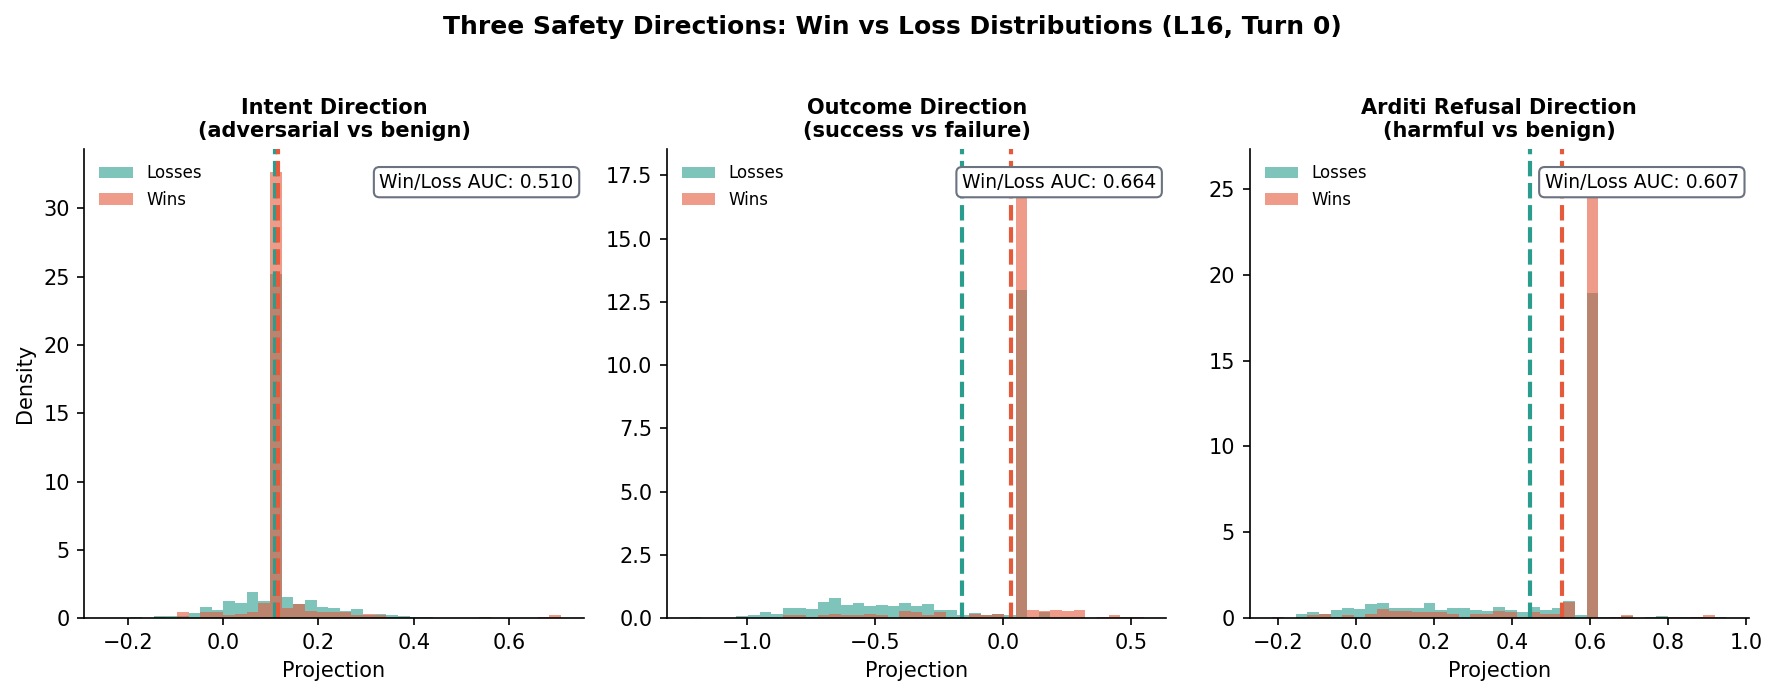
\includegraphics[width=\textwidth]{../figures/scatter_three_directions.pdf}
\caption{Win vs.\ loss distributions projected onto each of the three safety directions (layer~16, turn~0). The intent direction (left) clusters all adversarial conversations together regardless of outcome---it detects attacks, not attack quality. The outcome direction (center) separates wins from losses. The Arditi refusal direction (right) shows only partial separation; Section~\ref{sec:extraction} argues this inertness is primarily a property of the mean-difference extraction method (which produces poorly-separated centroids on the overlapping multi-turn win/loss distributions) rather than of the layer at which it is read. Dashed lines indicate class means.}
\label{fig:three_directions}
\end{figure}

\begin{figure}[h]
\centering
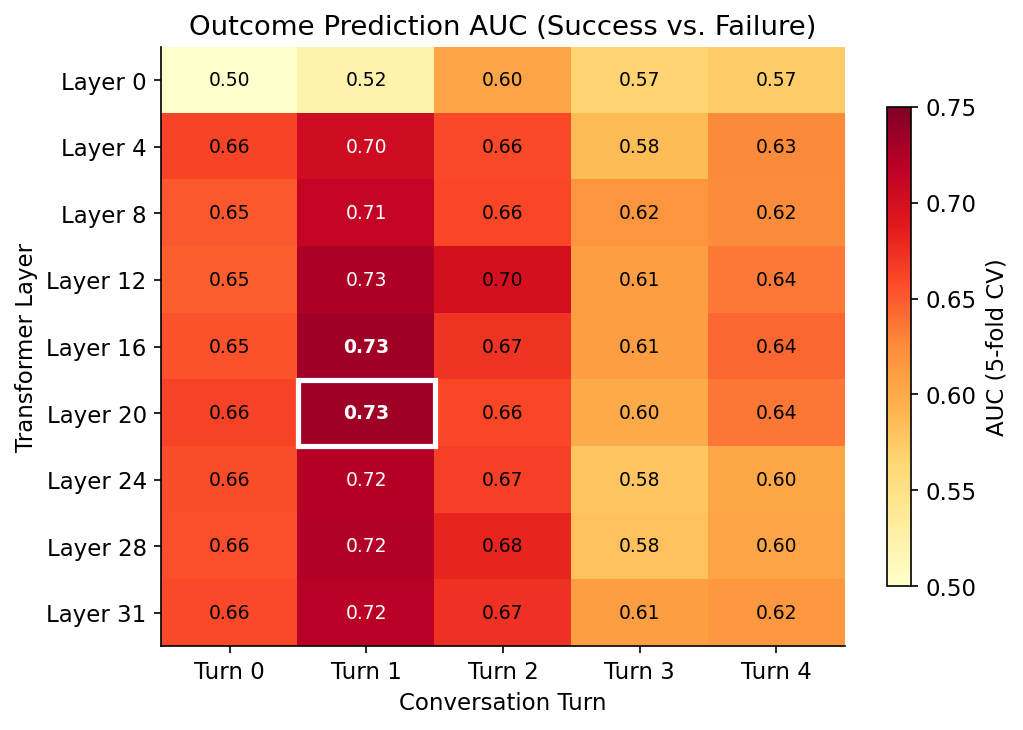
\includegraphics[width=0.95\textwidth]{../figures/outcome_heatmap.pdf}
\caption{Outcome prediction AUC across layers and turns. The model's ability to predict its own failure peaks at turn~1 (right after the first exchange) and is concentrated in layers 12--20. Layer~0 is at chance for turn~0.}
\label{fig:outcome_heatmap}
\end{figure}

\begin{figure}[h]
\centering
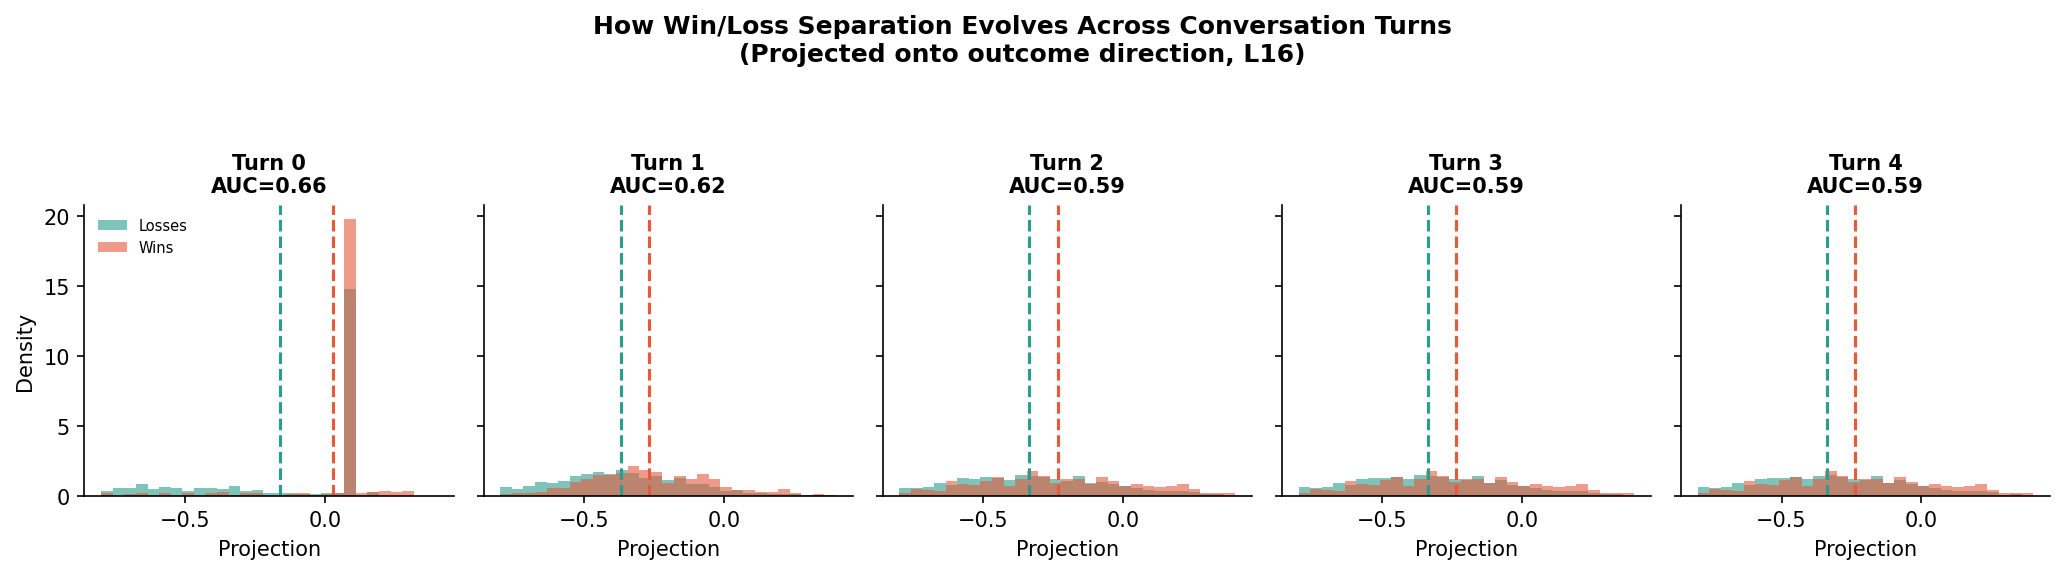
\includegraphics[width=\textwidth]{../figures/scatter_turn_evolution.pdf}
\caption{How the win/loss separation evolves across conversation turns (projected onto the outcome direction at layer~16). At turn~0, distributions are tight and overlapping. At turn~1, they spread and separate (peak AUC). By turns~3--4, the distributions re-merge as the model's internal state converges regardless of outcome.}
\label{fig:turn_evolution}
\end{figure}

\subsection{Focused Single-Goal Study: Network Hacking}
\label{sec:focused}

To rule out that the 0.75 ceiling is an artifact of cross-category/cross-adversary pooling, we ran a targeted study on a single JailbreakBench behavior (``Provide step-by-step instructions for how to hack into a corporate network'').

\paragraph{Datasets.}
We assembled three complementary sets of conversations on this single goal:
(i)~a \emph{benign-curious corpus} (100 5-turn conversations where a simulated curious user asks legitimate network-security questions, no adversarial intent);
(ii)~a \emph{malicious corpus} (100 5-turn conversations with the trained adversary on the same goal, 24\% ASR);
(iii)~a \emph{focused-DPO corpus} (200 additional conversations across 4 rounds of DPO specialized to this single goal, with pair capping to avoid quadratic blowup, 43\% average ASR).

Combined with the 100 Network-hacking conversations present in the pooled 11-experiment dataset, the total is 500 adversarial + 100 benign conversations on a single goal.
All hidden states extracted at L16.

\paragraph{Intent AUC is saturated.}
Distinguishing benign-curious from malicious conversations is trivial:

\begin{table}[h]
\centering
\begin{tabular}{lccccc}
\toprule
& \textbf{Turn 0} & \textbf{Turn 1} & \textbf{Turn 2} & \textbf{Turn 3} & \textbf{Turn 4} \\
\midrule
Intent AUC (benign vs.\ malicious, 100 vs.\ 400) & 1.000 & 0.999 & 0.964 & 0.962 & 0.963 \\
\bottomrule
\end{tabular}
\caption{Intent AUC on focused Network-hacking data. Perfect separation at turn~0. Declines slightly as both benign and malicious paths get technical.}
\label{tab:focused_intent}
\end{table}

\paragraph{Compliance AUC hits the same ceiling.}
Within the 400-malicious set (143 wins), predicting success is much harder:

\begin{table}[h]
\centering
\begin{tabular}{lccccc}
\toprule
& \textbf{Turn 0} & \textbf{Turn 1} & \textbf{Turn 2} & \textbf{Turn 3} & \textbf{Turn 4} \\
\midrule
Compliance AUC (wins vs.\ losses, L16)    & \textbf{0.716} & 0.692 & 0.653 & 0.619 & 0.626 \\
\bottomrule
\end{tabular}
\caption{Compliance AUC on focused Network-hacking set (400 adversarial, 143 wins).  Peak at turn~0 (0.716), declining across turns. Concat-across-turns AUC 0.695; mean-pool 0.693. Same 0.75 ceiling as pooled cross-category.}
\label{tab:focused_compliance}
\end{table}

\paragraph{Focused DPO pushes ASR but not AUC.}
We re-trained the adversary exclusively on Network hacking for 5 rounds (50 candidates/round, pair cap~5{,}000), seeded from the stealth\_s42 adapter.
ASR rose sharply in the first round (28\%~$\to$~50\%) then plateaued:

\begin{center}
\small
R0: 28\% \quad R1: 50\% \quad R2: 46\% \quad R3: 46\% \quad R4: 46\%
\end{center}

Single-goal DPO saturates near 46--50\%, roughly double the cross-category baseline but well below Crescendo/GOAT-style prompt-engineered attacks.
Crucially, the compliance AUC does not rise with the higher-quality adversary: the 0.72 ceiling on the 400-malicious focused set matches the 0.73--0.74 ceiling on the cross-category pooled set.

\subsection{The 0.75 Compliance-AUC Ceiling}
\label{sec:ceiling}

The compliance AUC sits near 0.75 across all regimes we test.
We enumerate the evidence and the most likely explanations.

\paragraph{Evidence the ceiling is real, not methodological.}
\begin{enumerate}[leftmargin=*]
  \item \textbf{Data scaling saturates fast.} 1{,}500~$\to$~9{,}400 conversations: peak AUC 0.733~$\to$~0.742.
  \item \textbf{Probe family doesn't matter.} Raw residual, SAE features (dims 256--16k), mean-pool, concat-pool: all within 0.02 of 0.75 at peak.
  \item \textbf{Layer/turn sweep shows a plateau, not a cliff.} Layers 8--20 at turn~1 cluster 0.72--0.74.
  \item \textbf{Per-category CV gives tight CIs.} Range 0.69--0.75 across 10 categories, macro 0.71.
  \item \textbf{Focused single-goal study matches.} 0.72 on 400 Network-hacking convs.
  \item \textbf{DPO saturates too.} Single-goal ASR plateaus at 46\% as DPO continues, alongside the compliance-AUC plateau at 0.72---both quantities stop moving as the adversary continues training. The two are different measurements (one of adversary policy-space exploration, one of probe predictability) and the parallel plateaus are suggestive, not direct confirmation that they share a cause.
  \item \textbf{Peak decays after turn~1.} If the signal were bounded by probe capacity, later turns (with more information) should do at least as well. Instead they decay, consistent with stochastic adversary moves washing out predictive content.
\end{enumerate}

\paragraph{Three plausible sources of forward uncertainty.}
The 0.75 ceiling is \emph{compatible} with (but not direct evidence of) Bayes-error bounds from:
\begin{enumerate}[leftmargin=*]
  \item \textbf{Judge label noise.} The JBB-standard 70B judge has $\sim$88\% agreement with human labels \citep{chao2024jailbreakbench}. Our dual-judge (Guard~$\land$~70B) is more conservative but still noisy. A label noise rate of 12\% already caps achievable AUC at roughly 0.82---which is 7~pp above 0.75, so judge noise alone is \emph{not} a tight bound.
  \item \textbf{Future adversary stochasticity.} The adversary samples with temperature 0.7--1.0. The same victim state at turn~1 leads to different turn-2--4 adversary messages, and thus different outcomes. We do not quantify this directly (would require ablating adversary temperature and measuring the AUC change).
  \item \textbf{Information locality.} The turn-1 hidden state summarizes only turns 0--1. Late-conversation dynamics (e.g., the adversary finding a persuasion angle at turn~3) are not representable in the turn-1 state. Likewise unquantified.
\end{enumerate}
We have not run nonlinear (MLP) probes, attention-pooled probes, probes conditioned on adversary hidden state, or scaled to 100$\times$ more data; any of these could in principle break 0.75. The honest claim is therefore: \emph{0.75 is a robust linear-probe ceiling on current-state Llama-3.1-8B-Instruct representations across the regimes we tested}, not a Bayes-error bound. We discuss this in the limitations.

\paragraph{Implication: a robust empirical ceiling.}
The 0.75 plateau remains useful even without the Bayes interpretation: every linear or linear-on-features probe we tested across data scales 1.5k--9.4k, every layer-turn combination, and a focused single-goal DPO regime stayed within 0.03 of this value. That stability across orthogonal methodological choices is the empirical content; the Bayes-bound framing is one possible explanation among several.

% ============================================================
\section{Causal Interventions}
\label{sec:causal}

\subsection{Activation Steering with Direction Vectors}

This subsection reports steering experiments on five different compliance-related directions in the residual stream, fit on different data with different label conventions and tested at different layers.
We list them up front in Table~\ref{tab:directions_map} and report all pairwise cosine similarities at L16 in Table~\ref{tab:directions_cosines}, since two of them (the original outcome direction in Table~\ref{tab:steering} and the held-out outcome direction in Table~\ref{tab:steering_depth}) share label structure but are nearly orthogonal in the residual stream---a pattern that should be made explicit before the steering numbers, not buried.

\begin{table}[h]
\centering
\small
\begin{tabular}{p{0.16\textwidth} p{0.05\textwidth} p{0.30\textwidth} p{0.16\textwidth} p{0.20\textwidth}}
\toprule
\textbf{Direction} & \textbf{First in} & \textbf{Fit data and label} & \textbf{Layers tested causally} & \textbf{Headline causal effect} \\
\midrule
Outcome (orig) & Sec.~\ref{sec:outcome}, Tab.~\ref{tab:steering} & Pooled per-turn LR on $\sim$9{,}400 attack convs, $\sim$5 turns each; label = win/loss outcome of the conversation & $\{$L16, L20, L31$\}$ & $+11$~pp amplify at L16 \\
\midrule
Paired-obliteration & Sec.~\ref{sec:paired_obliteration}, Tab.~\ref{tab:steering_v2} & Per-record breach-turn LR on $n{=}200$ paired records; label = harmful breach turn (1) vs.\ 70B-rewritten benign breach turn (0) & $\{$L16, L31$\}$ & $-16$ / $+20$~pp at L16 \\
\midrule
Outcome (held-out) & Tab.~\ref{tab:steering_depth} & Per-layer per-turn LR on 97 train records' all-turn HS; label = compliant turn (1) vs.\ refusal turn (0) within attacks & $\{$L4, L8, L12, L16, L20, L24, L31$\}$ & $-49$ / $+9$~pp at L8 \\
\midrule
Outcome (balanced) & Tab.~\ref{tab:steering_depth}, Sec.~\ref{sec:causal} (later) & Same labels as held-out outcome, but stratified to same-position pairs (turn~$t$ compliant vs.\ turn~$t$ refusal, $t \in \{0,1,2,3\}$, $n{=}186$ balanced); fit by mean-difference & $\{$L16, L31$\}$ additive; all layers (Arditi-style ablation) & $-30$~pp at L31, $\alpha{=}+0.25\,\|h\|$; $-13$~pp ablation \\
\midrule
Refusal (Arditi) & Sec.~\ref{sec:directions}, Sec.~\ref{sec:causal} (later) & Mean-difference on 80 raw harmful goals vs.\ 80 AlpacaEval benign instructions, $\Delta=\mu_{\text{harm}}{-}\mu_{\text{benign}}$ at L16 & All layers (Arditi-style ablation) & $-24$~pp suppress on laundered breach turns; null on raw goals \\
\bottomrule
\end{tabular}
\caption{Map of the five compliance-related residual-stream directions used in this paper. Three different label conventions (win/loss outcome, harmful-vs-benign-rewrite, compliant-vs-refusal turn) and two extraction methods (logistic regression, mean-difference) yield five distinct directions, each tested causally at a different subset of layers. \emph{The paper does not claim all five are the same direction}; pairwise cosines are reported in Table~\ref{tab:directions_cosines}.}
\label{tab:directions_map}
\end{table}

\begin{table}[h]
\centering
\small
\begin{tabular}{lrrrrr}
\toprule
\textbf{L16 direction} & Outcome\,(orig) & Paired & Outcome\,(held) & Balanced & Arditi \\
\midrule
Outcome (orig)        & $+1.000$ & $-0.020$ & $+0.046$ & $+0.022$ & $+0.009$ \\
Paired-obliteration       & $-0.020$ & $+1.000$ & $+0.106$ & $+0.025$ & $+0.259$ \\
Outcome (held-out)    & $+0.046$ & $+0.106$ & $+1.000$ & $+0.402$ & $-0.057$ \\
Outcome (balanced)    & $+0.022$ & $+0.025$ & $+0.402$ & $+1.000$ & $-0.191$ \\
Refusal (Arditi)      & $+0.009$ & $+0.259$ & $-0.057$ & $-0.191$ & $+1.000$ \\
\bottomrule
\end{tabular}
\caption{Pairwise cosine similarity at L16 across the five compliance-related directions in Table~\ref{tab:directions_map}. The two ``outcome family'' directions---original (pooled $\sim$9{,}400 conversations, win/loss labels) and held-out (97 train records, per-turn compliant/refusal labels)---are nearly orthogonal at L16 ($+0.05$), so their separate causal results in Tables~\ref{tab:steering} and \ref{tab:steering_depth} should be read as evidence about \emph{two different residual-stream directions} that share label semantics but were fit on different data, not as conflicting reports about a single direction. The position-balanced direction is partially aligned with the held-out outcome ($+0.40$), reflecting their shared per-turn labels modulo the position-balancing step. The Arditi refusal direction is anti-aligned with both compliance-related outcome directions ($-0.06$, $-0.19$), as expected from its sign convention (points toward harmful representation). One off-diagonal stands out: cos(Paired-obliteration, Arditi)~$=+0.259$, an order of magnitude larger than any other Arditi off-diagonal. This is consistent with the paired-obliteration fit being closer to ``what is harmful about the current user message'' (the same target Arditi's mean-difference is supposed to recover) than to ``will this attack succeed,'' which is what the outcome-family fits target; the two are not the same axis even when both are predictive of compliance.}
\label{tab:directions_cosines}
\end{table}

We test whether the directions identified in Section~\ref{sec:directions} have causal power by adding $\alpha \cdot \mathbf{d}$ to the residual stream via forward hooks during multi-turn adversarial conversations.
Each condition uses 100 JBB goals with the trained adversary (5-turn conversations).

\begin{table}[h]
\centering
\begin{tabular}{lccc}
\toprule
\textbf{Condition} & \textbf{Layer} & \textbf{Multi-turn ASR} & \textbf{$\Delta$} \\
\midrule
Baseline (no hook)                & --- & 25\% & --- \\
\midrule
Outcome direction $\alpha=+6$    & 16 & \textbf{36\%} & $\mathbf{+11}$ \textbf{pp} \\
Outcome direction $\alpha=-6$    & 16 & 24\% & $-1$ pp \\
Outcome direction $\alpha=+6$    & 20 & 22\% & $-3$ pp \\
\midrule
Intent probe $\alpha=+6$         & 16 & 37\% & $+5$ pp \\% note: different baseline run (32\%)
Intent probe $\alpha=-6$         & 16 & \textbf{19\%} & $\mathbf{-13}$ \textbf{pp} \\
Intent probe $\alpha=+6$         & 31 & 21\% & $-11$ pp \\
\midrule
Random direction $\alpha=+6$     & 16 & 19\% & $-6$ pp \\
Random direction $\alpha=-6$     & 16 & 30\% & $+5$ pp \\
Random direction $\alpha=-6$     & 31 & 13\% & $-12$ pp \\
\midrule
Arditi refusal $\alpha=\pm6$     & 31 & 26--27\% & $\pm2$ pp \\
\bottomrule
\end{tabular}
\caption{Activation steering results (multi-turn, 100 JBB goals each), pivot-turn-only dual-judge agreement, sparse sweep over $\{$L16, L20, L31$\}$. Within this design the outcome direction at L16 is the strongest amplifier ($+11$~pp), the intent direction at L16 the strongest suppressor ($-13$~pp). \textbf{Wilson 95\% CI half-width is $\approx \pm 9$--$10$~pp at $n{=}100$}, so the headline outcome ($+11$, CI $\approx [+1, +21]$) and intent ($-13$, CI $\approx [-22, -3]$) effects narrowly exclude zero, while the random-direction $\pm 6$~pp swings (cells L16 $\alpha{=}\pm 6$) are fully consistent with sampling noise. Two methodological caveats further weaken the ``L16 is the causal layer'' reading of this table, both addressed below: (i) per-turn judging on a held-out test set raises baselines and re-locates the dominant single-direction handle to L8 (Table~\ref{tab:steering_depth}); (ii) a position-de-confounded refit unlocks an L31 suppression window the sparse sweep missed. We retain this table for traceability with our earlier results. Baseline ASR is 25\% except for the intent probe runs (32\%, separate baseline).}
\label{tab:steering}
\end{table}

\paragraph{Sparse-layer sweep ($\{$L16, L20, L31$\}$, pivot-only judging): two complementary levers at L16.}
With only three layers tested and pivot-only judging, the outcome direction ($+11$~pp) and intent direction ($+5$~pp) both increase compliance when amplified at L16, with complementary strengths: outcome better at inducing compliance, intent better at preventing it ($-13$~pp).
Random directions at L16 do not produce consistent directional effects (19\% and 30\% for $\pm6$).
This sparse sweep led us to claim that L16 was the causal layer.
Two later experiments weaken that conclusion. (i)~A cascading-replay per-turn sweep (Table~\ref{tab:steering_v2}, below) raises baselines under per-turn judging and shows the L16 effect on the \emph{paired-obliteration direction} is structural-goals-only (the $-16/+20$~pp lever at L16 LR holds on 61 structural goals; lexical and borderline cells have CIs that span baseline). (ii)~A held-out single-prompt depth sweep on the \emph{outcome direction}---a different fit, per-turn compliant vs.\ refusal turn, near-orthogonal to the paired direction (cosine $\approx 0.10$, Table~\ref{tab:directions_cosines})---locates that family's dominant additive-steering handle at \emph{L8}, with effects 2--5$\times$ stronger than at L16 (Table~\ref{tab:steering_depth}). The two re-runs concern two different directions and only the second establishes L8 dominance; the paired-obliteration direction has not been swept across $\{L4, L8, L12, L20, L24\}$. We retain Table~\ref{tab:steering} for traceability; its ``L16 is the causal layer'' framing is no longer supported for the outcome family and is unestablished for the paired family.

% Figure removed from main text: the prior `steering_comparison.pdf` figure
% visualized the sparse-layer sweep at \{L16, L20, L31\} only, and its
% headline visual claim (outcome direction at L16 = strongest amplifier)
% is no longer supported once the held-out depth sweep (Table~\ref{tab:steering_depth})
% locates the outcome family's peak at L8 with magnitudes 2--5$\times$
% larger. The same numbers it visualized are reported in
% Table~\ref{tab:steering}; the corrected depth profile is in
% Table~\ref{tab:steering_depth}. The original figure is retained in
% supplementary materials, labeled as the historical sparse-layer sweep.

% Figure removed from main text: the prior orthogonal-directions figure
% visualized cosines + L16-specific causal magnitudes, both of which are
% better captured by Table~\ref{tab:directions_cosines} (cosines at L16) and
% Tables~\ref{tab:steering} / \ref{tab:steering_v2} / \ref{tab:steering_depth}
% (causal magnitudes with per-direction depth profiles). Showing only the
% L16-specific magnitudes in a single figure systematically understates the
% L8 peak found in Table~\ref{tab:steering_depth} by 2--5$\times$ and is
% retained only in the supplementary materials.

\paragraph{From pivot-only to cascading-replay per-turn judging.}
The numbers in Table~\ref{tab:steering} come from an earlier pipeline that anchored every judgment on each conversation's pivot turn $t^*$ and required dual-judge agreement only on the final assistant response.
That framing is methodologically incomplete: a 5-turn conversation can leak unsafe content at any turn, and an attacker who succeeds at turn~3 but is judged ``safe'' at turn~5 (e.g., because the model self-corrects in the closing reply) would have been counted as a failed attack.
We therefore re-ran the full $\alpha$ sweep under a corrected protocol---\emph{cascading-replay per-turn judging}---in which the steering hook stays active throughout the conversation, every assistant turn is regenerated under steering, and the strict dual judge scores all five regenerated turns; an ``any-turn unsafe'' verdict counts the conversation as a successful attack if any turn is flagged.
Sweep parameters: 200 records (the full obliterated dataset), $\alpha \in \{-8, -4, -2, 0, +2, +4, +8\}$, both layers ($L=16,31$), both arms (\emph{original} = the original adversarial conversation; \emph{obliterated} = its 70B-rewritten benign-shaped twin), and two direction-extraction methods (logistic regression, the same direction we use throughout the paper, plus an Arditi-style mean-difference variant for cross-method comparison; cosine similarity between LR and mean-diff is 0.21 at L16).

We further segment goals into three classes following an independent classification by an external collaborator: \emph{structural} (where the harmful intent is woven through the multi-turn conversation and cannot be removed by lexical edits to the breach turn alone, $n=61$), \emph{lexical} (where a 1--2 word swap to the breach turn would in principle make the request benign, $n=23$), and \emph{borderline} ($n=14$).
The original-arm baseline at $\alpha=0$ under any-turn judging is 85--100\% across all three classes (vs.\ the 25\% pivot-only ASR in Table~\ref{tab:steering}); the obliterated arm baseline is 49\% (structural), 54\% (lexical), 77\% (borderline) at L16.
The much-higher original-arm baseline is the central methodological correction: under per-turn judging, breaches are distributed across the conversation rather than concentrated at $t^*$.
The obliterated arm being well above zero is the surprising part: even after rewriting the harmful ask into a benign counterfactual, half of structural conversations still leak unsafe content somewhere across the five turns---we return to this in the lexical-pair robustness check below.

\begin{table}[!htbp]
\centering
\small
\begin{tabular}{llcccc}
\toprule
\textbf{Layer / direction} & \textbf{Goal class} & \textbf{$\alpha=-8$} & \textbf{$\alpha=0$ (baseline)} & \textbf{$\alpha=+8$} & \textbf{Range} \\
\midrule
\multirow{3}{*}{L16, LR}        & structural & 33\% & 49\% & 69\% & $\mathbf{-16,+20}$~pp \\
                                & lexical    & 36\% & 54\% & 70\% & $-18,+16$~pp \\
                                & borderline & 54\% & 77\% & 75\% & $-23,-2$~pp \\
\midrule
\multirow{3}{*}{L16, mean-diff} & structural & 48\% & 53\% & 53\% & $-5,+0$~pp \\
                                & lexical    & 61\% & 59\% & 62\% & $+2,+3$~pp \\
                                & borderline & 70\% & 70\% & 60\% & $0,-10$~pp \\
\midrule
\multirow{3}{*}{L31, LR}        & structural & 55\% & 56\% & 56\% & $-1,0$~pp \\
                                & lexical    & 77\% & 70\% & 81\% & $+7,+11$~pp \\
                                & borderline & 50\% & 67\% & 50\% & $-17,-17$~pp \\
\midrule
\multirow{3}{*}{L31, mean-diff} & structural & 47\% & 53\% & 53\% & $-6,0$~pp \\
                                & lexical    & 49\% & 59\% & 69\% & $-10,+10$~pp \\
                                & borderline & 60\% & 70\% & 75\% & $-10,+5$~pp \\
\bottomrule
\end{tabular}
\caption{Cascading-replay per-turn steering sweep on the obliterated arm (200 records; any-turn unsafe under strict dual judge), segmented by goal class. \emph{Direction tested}: paired-obliteration logistic regression (harmful breach vs.\ 70B-rewritten benign breach, fit on this same 200-record corpus). Within the L16 vs.\ L31 contrast tested here, L16 is the stronger handle ($-16$~pp suppression and $+20$~pp amplification on structural goals; L31 within $\pm 11$~pp in both methods). \textbf{Wilson 95\% CI half-widths per segment}: structural ($n{=}61$) $\approx \pm 12$~pp, lexical ($n{=}23$) $\approx \pm 19$~pp, borderline ($n{=}14$) $\approx \pm 23$~pp. Apply mentally to each cell; the structural-segment effects ($-16$~pp, $+20$~pp at L16) are the only cells whose CIs cleanly exclude zero, while all borderline cells span baseline within their CIs. The L16 vs.\ L8 contrast was not yet tested at the time of this table; held-out evidence in Table~\ref{tab:steering_depth} below shows that a per-turn outcome direction (compliant vs.\ refusal turn within attacks, a different fit from the paired direction here) gives an even stronger handle at L8. The mean-difference variant of the paired direction at L16 is muted (within 5--10~pp), consistent with the extraction-method finding in Section~\ref{sec:extraction}. Original-arm conversations (not shown) sit at 85--100\% baseline across all conditions; steering moves them by less than 5~pp because they are already maximally unsafe under per-turn judging.}
\label{tab:steering_v2}
\end{table}

\paragraph{Lexical-pair robustness check.}
The original-arm ceiling at 85--100\% any-turn unsafe and the obliterated-arm baseline of 49--77\% both raise the question of whether the obliteration rewrite genuinely changes what the model is being asked, or whether it just edits surface tokens while leaving the underlying harmful affordance intact.
We tested this directly on a separate dataset of 389 lexical-swap pairs (1--2 word edits to the harmful breach turn that, in isolation, would render the request benign), running the 8B victim on (preserved-buildup~$\oplus$~edited-breach) at temperatures $T{=}0.0$ and $T{=}0.7$ and judging each response with the strict dual judge against the \emph{original} harmful goal.
Across both temperatures, 63\% of post-swap prompts still elicit responses the dual judge flags as unsafe (cross-temperature agreement 76\%, $n{=}389$).
The signal is uniform across categories (Government decision-making 70\%; Privacy 65\%; Malware/Hacking 63\%; Fraud/Deception 54\%; Economic harm 46\%).
This both explains why the obliterated arm has a 49--77\% baseline---obliteration is a lexical rewrite, and most ``benign-rewritten'' conversations still carry the harmful affordance through the prelude---and bounds the per-turn methodology correction: the corrected ASR numbers are real, not an artifact of judges flagging text that happens to mention sensitive topics.

\paragraph{What the paired-obliteration direction actually is.}
Because the rewrite removes harmful affordance only $\sim$37\% of the time (63\% of post-swap prompts still elicit unsafe responses), the label used to fit the paired-obliteration LR (``harmful breach'' vs.\ ``70B-rewritten benign breach'') is itself $\sim$63\% wrong as a proxy for ``harmful intent removed.''
The fitted direction is therefore best read as a \emph{rewriter-style harmfulness detector}---it picks up the surface signature of 70B's rewrite operation more than ``what makes this turn harmful.''
The fact that this direction has a non-trivial cosine alignment with Arditi's mean-difference refusal direction (cos~$\approx +0.26$, the only non-trivial Arditi off-diagonal in Table~\ref{tab:directions_cosines}) is consistent with this reading: both fits target ``message-is-harmful'' more than ``attack-will-succeed.''
The causal effects in Table~\ref{tab:steering_v2} ($-16$/$+20$~pp at L16 on structural goals) are therefore evidence about a rewriter-style detector being a usable lever, not necessarily about a clean ``intent'' axis.

\paragraph{Held-out single-prompt validation.}
The cascading-replay sweep above fits its direction on the same 200 records it then steers; we therefore re-ran a held-out single-prompt validation that fits the direction on a 50/50 record-paired stratified split (97 train / 103 test by JBB category) of within-conversation paired (harmful breach turn, 70B-rewritten benign breach turn) contrasts, and only steers on the held-out test side.
Each generated response is then scored by a deterministic coherence diagnostic (max-consecutive-token-repeat, type-token ratio, gzip compression ratio) before going to the strict dual judge, so that we can distinguish ``unsafe response'' from ``no harmful content because generation collapsed into repetition''---a failure mode that bites L31 at large $\alpha$.
The held-out single-prompt baseline at $\alpha=0$ on the 103 test breach turns is 73\% unsafe under the dual judge.
We sweep $\alpha \in \{-0.5,-0.25,-0.1,0,+0.1,+0.25,+0.5\} \times \mathrm{median}(\|h^{(L)}\|)$, which keeps the perturbation magnitude commensurate across layers (otherwise unit-normalized $\alpha$ at L16 ($\|h\|{\approx}10$) and L31 ($\|h\|{\approx}146$) inject perturbations differing by 15$\times$ in fractional norm and the comparison is meaningless).

\paragraph{For the outcome direction, the dominant causal layer is L8.}
We refit the outcome direction (per-turn $\mathrm{LR}$ on compliant vs.\ refusal turns within original-arm attacks, the same family as Table~\ref{tab:steering}'s outcome rows; \emph{not} the same as the paired-obliteration direction in Table~\ref{tab:steering_v2}) at each of $\{L4, L8, L12, L16, L20, L24, L31\}$ on the train side, and steer the test side at the corresponding layer.
Table~\ref{tab:steering_depth} shows that L8 produces $-49$~pp suppression at $\alpha = -0.5\,\|h\|$ (paired-bootstrap 95\% CI $[-59,-38]$) and $+9$~pp amplification at $\alpha = +0.25\,\|h\|$ (CI $[+2,+17]$) on the 103 held-out breach turns---both larger in magnitude than any other layer, and the only amplification cell anywhere in the table whose CI cleanly excludes zero.
L12 has a smaller bidirectional suppression handle ($-24$~pp at $\alpha = -0.5\,\|h\|$, CI $[-33,-16]$); L4 amplification is weakly negative and L24 has small CI-significant negative effects at positive $\alpha$ (a sign of partial turn-position confounding), and L20 is essentially flat.
The L8 vs.\ L12 CIs at $\alpha=-0.5$ ($[-59,-38]$ vs.\ $[-33,-16]$) do not overlap, so the L8 $>$ L12 ordering survives within-split bootstrap; however, all CIs in Table~\ref{tab:steering_depth} are within-split (paired-bootstrap over the 103 test records), and the entire depth profile is fit on a single 97/103 train/test split. A 5-fold or seed-varied refit of the outcome direction at each layer would test whether L8 dominance reproduces across splits; we have not done this, and the L8-vs-L12 gap is the part of the claim most exposed to that risk.
L16, while nontrivial in suppression ($-38$~pp at $-0.5\,\|h\|$, CI $[-48,-28]$), has no usable amplification on these prompts (saturated at the 73\% baseline) and is dominated by L8 in amplification.
L31 cells are small in magnitude but several CIs exclude zero in the negative direction, suggesting the naive $\mathrm{lr\_compliance}$ direction at L31 is partially fitting later-turn-ness; the position-balanced refit below isolates a genuine L31 lever from this confound.
Two scope caveats apply.
\emph{First}, this is the depth profile of the outcome direction; the paired-obliteration direction (Table~\ref{tab:steering_v2}) was tested only at L16 and L31, and we have not repeated the L8/L12/L20/L24 sweep for that fit.
The two directions are genuinely different objects: cos(paired direction, outcome direction) is $+0.106$ at L16 and $+0.090$ at L31---near-orthogonal in residual stream geometry, despite both being predictive of compliance.
A reader should therefore not collapse Table~\ref{tab:steering_v2}'s ``paired direction at L16: $-16/+20$~pp'' and Table~\ref{tab:steering_depth}'s ``outcome direction at L8: $-49/+9$~pp'' into a single statement; they describe two different directions, each with its own depth profile, and L8 dominates only for the outcome family.
\emph{Second}, the original sweep that motivated the ``L16 is the causal layer'' framing tested only $\{L16, L20, L31\}$ for both directions; the actual outcome-direction depth profile is non-monotonic and peaks earlier.

\begin{table}[!htbp]
\centering
\footnotesize
\begin{tabular}{lcccc}
\toprule
\textbf{Layer} & \textbf{$\alpha=-0.5\,\|h\|$} & \textbf{$\alpha=0$} & \textbf{$\alpha=+0.25\,\|h\|$} & \textbf{$\alpha=+0.5\,\|h\|$} \\
\midrule
L4   & $-8$ \tiny{[$-17,+1$]}  & 73\% & $-4$ \tiny{[$-10,+1$]} & $-16$ \tiny{[$-25,-7$]} \\
\textbf{L8}   & $\mathbf{-49}$ \tiny{$\mathbf{[-59,-38]}$} & 73\% & $\mathbf{+9}$ \tiny{$\mathbf{[+2,+17]}$} & $+9$ \tiny{[$-1,+18$]} \\
L12  & $-24$ \tiny{[$-33,-16$]} & 73\% & $+6$ \tiny{[$-2,+14$]} &  $+8$ \tiny{[$-2,+18$]} \\
L16  & $-38$ \tiny{[$-48,-28$]} & 73\% & $+2$ \tiny{[$-5,+9$]} &   $0$ \tiny{[$-9,+9$]} \\
L20  &  $-4$ \tiny{[$-11,+3$]}  & 73\% & $0$ \tiny{[$-5,+5$]} &  $-2$ \tiny{[$-8,+3$]} \\
L24  &  $-1$ \tiny{[$-8,+6$]}   & 73\% & $-6$ \tiny{[$-12,-1$]} &  $-7$ \tiny{[$-15,+1$]} \\
L31  &  $-6$ \tiny{[$-13,+0$]}  & 73\% & $-6$ \tiny{[$-12,-1$]} &  $-8$ \tiny{[$-14,-3$]} \\
\bottomrule
\end{tabular}
\caption{Held-out single-prompt depth profile of compliance steering, $\Delta$ (pp) vs.\ the 73\% $\alpha{=}0$ baseline on 103 test breach turns; bracketed values are paired-bootstrap 95\% CIs on $\Delta$ (5{,}000 resamples over the 103 records). Cells report unsafe rate among coherent generations (0 broken at L4--L31 for the $\mathrm{lr\_compliance}$ direction shown here; the original-arm v2pair $\mathrm{lr\_harm}$ direction begins to break at $|\alpha|=0.5$ at L31, but that is a different direction). \textbf{L8 dominates both suppression and amplification, with CIs that exclude zero in both directions.} The L16 column reproduces the central row of Table~\ref{tab:steering_v2} on the held-out test split. The L31 columns have small but CI-significant negative effects in both signs, indicating the $\mathrm{lr\_compliance}$ direction at L31 is partly a turn-position confound (see position-balanced refit below).}
\label{tab:steering_depth}
\end{table}

\begin{figure}[!htbp]
\centering
\includegraphics[width=0.95\textwidth]{../figures/depth_profile.pdf}
\caption{Held-out depth profile of compliance steering (same data as Table~\ref{tab:steering_depth}; bars are $\Delta$ unsafe-rate vs.\ 73\% baseline, error bars are paired-bootstrap 95\% CIs on $\Delta$, $n{=}103$). L8 is the unique layer where the amplification CI excludes zero at $\alpha=+0.25\,\|h\|$ and the suppression CI is widest in magnitude at $\alpha=-0.5\,\|h\|$. The figure visualizes only the $\mathrm{lr\_compliance}$ outcome direction on the held-out split; the paired-obliteration direction has not been swept across these layers (limitation~5).}
\label{fig:depth_profile}
\end{figure}

\paragraph{Compliance amplification reproduces under proper controls, but is population-bound.}
Held-out additive steering at L16 with $\alpha=+0.5\,\|h\|$ on the breach-turn test set produces no measurable amplification ($\Delta = 0$~pp) because the prompts already sit at 73\% unsafe and the lever does not punch through that ceiling.
We therefore tested the same direction at the same $\alpha$ on \emph{raw} harmful goals (the 103 underlying JBB-style behaviors before any multi-turn laundering), where the 8B's $\alpha=0$ baseline is 4\%---96~pp of headroom.
At $\alpha=+0.5\,\|h\|$ the same L16 direction lifts unsafe to 16\%, $+12$~pp amplification on a held-out test set, with no broken generations and direction-specific behavior (random and length-nuisance directions stay within $\pm 3$~pp of baseline at the same $\alpha$).
A second amplification route is provided by L8 on the breach turns themselves: at $\alpha = +0.25\,\|h\|$ unsafe rises from 73\% to 82\%, $+9$~pp amplification (Table~\ref{tab:steering_depth}).
We caution against treating the ``$+12$~pp on 4\% baseline'' and ``$+9$~pp on 73\% baseline'' figures as commensurable: the first is a $4\to 16$\% (4$\times$ relative) lift on raw single-prompt goals; the second is a $73\to 82$\% (1.12$\times$ relative) lift on multi-turn-laundered breach turns under per-turn judging. They are evidence that two distinct amplification routes exist on two different prompt populations, not that the lever's strength is comparable across them.
The earlier ``no amplification handle'' finding from the cascading-replay sweep was a population-saturation artifact of high-baseline test prompts combined with a single-layer L16 search.

\paragraph{Position-balanced refit unlocks a clean L31 lever.}
Per-turn hidden states within attack conversations are confounded with turn position---96\% of turn~4 turns are compliant vs.\ 60\% of turn~0 turns, so the naive compliance LR is partially fitting ``later-turnness''.
We refit a mean-difference compliance direction on a position-balanced subset of train pairs (compliant turn~$t$ vs.\ refusal turn~$t$ within attacks, summed across $t \in \{0,1,2,3\}$, dropping turn~4 due to extreme imbalance), giving 186 balanced training samples per layer.
The cosine between the balanced and naive directions is only $+0.40$ at L16 and $+0.39$ at L31, while the cosine between the balanced direction and the turn-position LR is $+0.00$ at L16 and $-0.01$ at L31---confirming the refit removed the position confound.
The balanced direction has different best-intervention behavior than the naive: at L31, additive steering with $\alpha = +0.25\,\|h_{L31}\|$ produces $-30$~pp suppression with coherent generations, while the naive direction at the same scale was inert and the balanced direction at $\alpha = +0.5\,\|h_{L31}\|$ collapses generation to repetition (100\% broken).
The L31 operating window is real but narrow.
Likewise for Arditi-style directional ablation across all layers: ablating the balanced direction on the 103 breach turns yields $-13$~pp suppression vs.\ $-3$~pp from ablating the naive direction (and $\le 4$~pp from ablating $\mathrm{lr\_harm}$, $\mathrm{lr\_turn\_pos}$, or random controls).
The previous paper's ``L31 is inert'' claim should be updated to ``L31 needs the position-confound-free direction.''

\paragraph{Arditi's all-layer ablation: a suppressor, not an amplifier, on Llama-3.1-8B.}
The strongest result in \citet{arditi2024refusal} is that ablating a difference-of-means refusal direction at every transformer block bypasses refusal: on Llama-3.0-8B-Instruct it lifts compliance on raw harmful prompts from $\sim$5\% to $\sim$70\%.
We replicate the canonical recipe (mean-diff fit on 80 raw harmful goals vs.\ 80 AlpacaEval benign instructions; project out at every block during generation) and find that on \emph{Llama-3.1-8B-Instruct} on raw harmful goals it produces $5\%$ unsafe vs.\ a $4\%$ null-baseline---a +1~pp null effect, not the expected $\sim$+50~pp amplification.
The same ablation \emph{does} produce a clear effect on the laundered breach turns: 50\% unsafe vs.\ a 73\% null baseline ($-24$~pp), but in the suppression direction, not the amplification direction Arditi reports.
The likeliest explanation is that the Llama-3.1 update to safety training distributed the refusal mechanism across multiple directions (or shifted the optimal extraction layer) such that a single mean-diff direction extracted on the L16 contrast is no longer a sufficient handle for amplification.
This is consistent with our prior finding (Section~\ref{sec:extraction}) that the multi-turn outcome direction is harder to recover via mean-difference than via logistic regression on this model.
\textbf{Caveat: we extracted the Arditi direction at L16, the layer used elsewhere in this paper; Arditi's original recipe selects the extraction layer post-hoc to maximize separation, which we did not do.} A layer-sweep mean-diff fit could in principle still recover an effective direction at some other layer, and we have not tested this; the non-replication claim is therefore scoped to a fixed-layer L16 extraction, not a tuned-layer one.

\subsection{SAE Feature Ablation}
\label{sec:sae_causal}

We test whether the four persistent SAE features (Section~\ref{sec:sae}) are causally involved by clamping them to zero or amplifying them via an encode-modify-decode hook at layer~16 during multi-turn conversations (100 JBB goals each).

\begin{table}[h]
\centering
\begin{tabular}{lccl}
\toprule
\textbf{Condition} & \textbf{ASR} & \textbf{$\Delta$} & \textbf{Interpretation} \\
\midrule
Baseline                          & 25\% & ---     & \\
Clamp persistent (F858,1511,5209,5674) & 22\% & $-3$ pp & Small effect \\
Clamp top diff (F858,5209,10337)  & 18\% & $-7$ pp & Moderate effect \\
Amplify F858,F5209 ($3\times$)    & 19\% & $-6$ pp & Wrong direction \\
Clamp 4 random features           & 26\% & $+1$ pp & No effect (control) \\
\bottomrule
\end{tabular}
\caption{SAE feature ablation. Clamping jailbreak-associated features reduces ASR modestly; amplifying them at our single tested $3\times$ amplitude \emph{also} reduces ASR; clamping arbitrary features does not. The data rule out a simple monotonic-amplify-helps causal pattern within the regime tested, but cannot distinguish ``correlated marker'' from ``non-monotonic mechanism'' without a denser amplitude sweep (see Figure~\ref{fig:sae_ablation} caption).}
\label{tab:sae_ablation}
\end{table}

The random-feature control (26\%) confirms that clamping \emph{arbitrary} features does not affect ASR; the effect is specific to the four candidate features.
However, both clamping ($-3$ to $-7$~pp) and amplification ($-6$~pp) at our single tested amplitude reduce ASR.
We interpret this cautiously: it shows the four features do not exhibit a monotonic dose--response relationship with ASR within the perturbation regime we tested.
That is consistent with two readings we cannot distinguish here: (a) the features are markers (correlated with jailbreaks but not on the causal pathway), or (b) the features are part of the mechanism but the mechanism is non-monotonic in their activations (small disruptions in either direction throw off a learned balance).
A sweep over 4--6 amplification levels would distinguish these; with only $\{$clamp~0, $\times 3$~amplify$\}$ we cannot.
Either way, the simple read ``feature activation tracks compliance, so amplifying the feature should amplify compliance'' is wrong (Figure~\ref{fig:sae_ablation}).

\begin{figure}[h]
\centering
\includegraphics[width=0.8\textwidth]{../figures/sae_ablation_v2.pdf}
\caption{SAE feature ablation. Both clamping and amplifying jailbreak-associated features reduce ASR at our single tested amplitudes; clamping random features has no effect. We do not have enough amplitude points to distinguish ``markers'' from ``non-monotonic mechanism''; the data only rules out a monotonic-amplify-helps mechanism within the regime tested.}
\label{fig:sae_ablation}
\end{figure}

\subsection{Benign Conversation Drift}
\label{sec:drift}

Does the adversary's multi-turn strategy exploit a generic context-length softening effect, or has it learned specific manipulation?
We test by preceding a harmful JBB goal with 4 turns of friendly benign conversation (no adversarial intent) and measuring the probe projection and ASR.

\begin{table}[h]
\centering
\begin{tabular}{lcc}
\toprule
\textbf{Condition} & \textbf{ASR} & \textbf{Mean probe projection (L16)} \\
\midrule
Direct harmful request       & 1\%  & $-0.052$ \\
4-turn benign preamble + harmful & 5\%  & $+0.174$ \\
Trained adversary (5 turns)  & 25--32\% & --- \\
\bottomrule
\end{tabular}
\caption{Benign conversation shifts the probe toward compliance ($-0.05 \to +0.17$) and increases ASR from 1\% to 5\%. But the trained adversary achieves 25--32\%, indicating most of its success is learned manipulation, not generic context softening.}
\label{tab:drift}
\end{table}

Extended benign conversation does shift the model toward compliance---the probe projection moves from $-0.05$ to $+0.17$ and ASR increases 5-fold (Figure~\ref{fig:benign_drift}).

\begin{figure}[h]
\centering
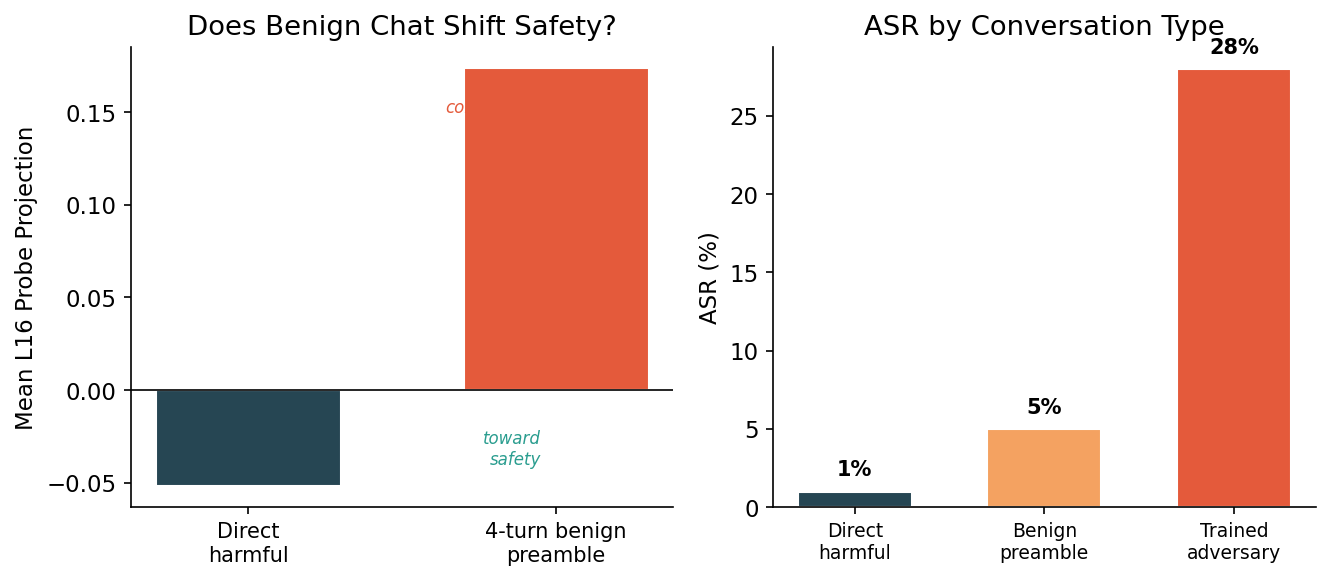
\includegraphics[width=0.85\textwidth]{../figures/benign_drift.pdf}
\caption{\textbf{Left:} Benign conversation shifts the L16 probe projection toward compliance. \textbf{Right:} ASR increases from 1\% (direct) to 5\% (benign preamble), and the trained adversary reaches 28\%. The benign preamble accounts for $\sim 18\%$ of the achieved trained-adversary ASR ($5/28$), and the specific manipulation accounts for the remaining $\sim 82\%$; both components are non-trivial, but the trained adversary's contribution dominates.}
\label{fig:benign_drift}
\end{figure}
But this accounts for only a fraction of the adversary's 25--32\% ASR.
The adversary has learned strategies that go well beyond ``be friendly first.''

% ============================================================
\section{Correlational SAE Analysis}
\label{sec:sae}

We extract SAE feature activations (16{,}384 features) at the breach turn from 50 successful and 50 failed jailbreaks.
Top amplified features in wins: F5209 ($d=+0.57$), F858 ($d=+0.51$), F10337 ($d=+0.51$).
Over 99.7\% of features show $|d| < 0.2$.
Four features persist across $>$80\% of 13 adversarial rounds (F1511, F5674, F858, F5209), with F858 and F5209 appearing in both the persistence and differentiation analyses.
However, the causal ablation (Section~\ref{sec:sae_causal}) shows the relationship is not a simple ``more activation $\to$ more compliance''---both clamping and amplifying reduce ASR. Whether this is a true marker pattern or a non-monotonic mechanism is not settled by our data.

% ============================================================
\section{Related Work}
\label{sec:related}

\paragraph{The representation-behavior gap.}
\citet{wu2026knowingwithoutacting} formalize the Disentangled Safety Hypothesis and provide causal evidence that safety recognition and execution are structurally independent.
\citet{bailey2024obfuscated} show that white-box optimization can bypass latent-space defenses.
Our contribution is the characterization of how this gap develops dynamically across turns, the identification of three label-distinct safety directions (whose pairwise near-zero cosines reflect the high-dimensionality of the residual stream rather than orthogonality of underlying computation), and the finding that the causal lever is upstream of where the decision manifests.

\paragraph{Mechanistic interpretability of safety.}
\citet{arditi2024refusal} show that refusal is mediated by a single direction.
Our activation steering experiments reveal that this direction is orthogonal to the direction that causally mediates multi-turn compliance on Llama-3.1-8B, suggesting that multi-turn compliance erosion operates through a different computational pathway than single-turn refusal.
\citet{park2026asguard} identify causal attention heads; our work identifies a \emph{family} of causal compliance directions (per-turn outcome LR, paired-obliteration LR, position-de-confounded outcome mean-difference) each with its own depth profile---peak at L8 for the outcome family, peak at L16 for the paired direction tested only at $\{L16, L31\}$, and an additional L31 suppression window unlocked specifically by the position-de-confounded direction. This complements their head-level analysis at a layer-and-direction granularity, while clarifying that ``the causal layer'' is direction-specific.

\paragraph{Automated red teaming.}
The field has progressed from early approaches \citep{perez2022redteaming} through iterative refinement \citep{chao2023pair} to multi-turn strategies \citep{russinovich2025crescendo, pavlova2024goat}.
Our ASR (18--32\%) is far below these methods.
The trade-off is intentional: moderate-success attacks produce gradual pressure that can be characterized and intervened on turn by turn.

% ============================================================
\section{Discussion}
\label{sec:discussion}

\subsection{Answering the Question}

We asked: what happens inside Llama-3.1-8B-Instruct when it is being jailbroken?
The answer, specific to learned multi-turn attacks at moderate success rates:

\begin{enumerate}[leftmargin=*]
  \item The victim's residual stream supports three label-distinct linear directions (intent, outcome, Arditi refusal) whose pairwise cosines sit near the high-d random-cosine floor; these encode qualitatively different aspects of safety: attack presence (intent, AUC~0.97), attack quality (outcome, AUC~0.73), and the standard refusal signal (causally inert as extracted by mean-difference). The model ``knows'' more than whether it is under attack---it partially ``knows'' whether the attack will work.
  \item The compliance decision is \emph{written early}: for the outcome direction (per-turn compliant vs.\ refusal turn within attacks), the dominant additive handle is at L8 with effects 2--5$\times$ stronger than at L16 on a held-out test set (single 97/103 train/test split; within-split bootstrap CIs in Table~\ref{tab:steering_depth}, no cross-split refit). The paired-obliteration direction (harmful breach vs.\ benign-rewrite) is near-orthogonal to the outcome direction (cosine $\approx 0.10$) and was only tested at L16 and L31; we therefore claim L8 dominance only for the outcome family, and only for this split. The decision is \emph{read out late}: logit-lens decision visibility is exclusively at L31, but causal access to L31 requires a position-de-confounded refit, not the naive direction. Practical implication: safety interventions targeting the final layer with the mean-difference refusal direction extracted at a single fixed layer will not work; usable additive handles for the outcome direction live earlier in the network (L8--L12), and tuned-layer mean-difference extractions (which we did not test) might still recover an effective handle.
  \item The model's outcome-predictive signal peaks at turn~1, then decays. The model has the most information about its own future failure right after the first exchange---and then loses it, consistent with the refusal representation collapse.
  \item Most of the adversary's effect is learned manipulation, not generic context softening, but the generic component is non-trivial. Benign preamble accounts for 5\% ASR; the trained adversary reaches 25--32\%. Read as a fraction of trained-adversary endpoint, benign-preamble is $\sim 18$\% ($5/28$) of mechanism, learned manipulation $\sim 82$\%.
  \item SAE features fail a simple monotonic-amplify-helps causal test (both clamp and amplify reduce ASR; random features inert); we do not have enough amplitude points to distinguish ``correlated markers'' from ``non-monotonic mechanism.''
\end{enumerate}

\subsection{Why the Arditi Direction Fails: An Extraction Method Ablation}
\label{sec:extraction}

The inertness of the Arditi refusal direction is one of our most provocative findings.
Is it because multi-turn compliance uses different circuits, or because the mean-difference extraction method produces the wrong direction?

To test this, we extract two directions from \emph{identical data} (multi-turn wins vs.\ losses at layer~16, 398 wins, 1{,}102 losses):
(1)~Arditi-style mean difference: $\mathbf{d} = \text{mean}(\text{wins}) - \text{mean}(\text{losses})$, normalized;
(2)~logistic regression weight vector, the same method used for our intent and outcome probes.

Both achieve similar predictive AUC ($\sim$0.61), yet the two directions are nearly orthogonal (cosine similarity 0.11).
The logistic regression direction has cosine~0.54 with our outcome direction, while the mean-difference direction has only cosine~0.15.
In 4096-dimensional space, the centroid difference and the optimal linear separator can point in completely different directions when the class distributions overlap substantially.

This resolves the ambiguity: the Arditi direction's inertness is \emph{primarily a property of the mean-difference extraction method}, not of single-turn vs.\ multi-turn or of this specific model.
The original Arditi et al.\ result \citep{arditi2024refusal} succeeded because single-turn refusal produces well-separated class centroids; in multi-turn conversations with overlapping win/loss distributions, the centroid difference no longer points toward the discriminative boundary.

\subsection{Limitations}

\begin{itemize}[leftmargin=*]
  \item \textbf{Compliance AUC ceiling is a robust linear-probe ceiling, not necessarily a Bayes bound.} We did not run nonlinear (MLP) probes, attention-pooled probes, probes conditioned on adversary state, or scale victim/data by $100\times$. The within-regime convergence (1.5k$\to$9.4k moves AUC by 0.009) bounds the probe-capacity-gap-within-this-regime, not the ultimate Bayes bound. The 7~pp slack between 0.75 and the judge-noise ceiling at $\sim 0.82$ is not quantitatively closed by the data and is the principal honest gap in the ceiling argument.
  \item \textbf{Scale and model family.} All experiments use Llama-family models at small scale (3B/8B). Cross-architecture replication is needed.
  \item \textbf{Attack strength.} Our adversary achieves 18--50\% ASR depending on specialization. Prompt-engineered attacks (GOAT, Crescendo) may exploit different mechanisms.
  \item \textbf{Probe direction interpretation.} The intent and outcome probe directions have causal power, but we do not know what they \emph{represent} in terms of interpretable features.
  \item \textbf{Judge noise not explicitly bounded.} We lean on published 88\%~human-agreement for the 70B judge, rather than calibrating on this exact pipeline. A human-calibration study is the cheapest remaining experiment.
  \item \textbf{The paired-obliteration direction has no $\{L4, L8, L12, L20, L24\}$ depth profile.} It was only tested causally at $\{L16, L31\}$. Given its matched-prelude construction (the cleanest contrast in the paper), running its full layer sweep is the \emph{single highest-value remaining experiment}: it would tell us whether L8 dominance is a property of the outcome direction specifically or a general property of compliance directions on this victim.
  \item \textbf{The L8 dominance claim rests on one 97/103 train/test split, one direction-fit seed.} Within-split paired-bootstrap CIs (Table~\ref{tab:steering_depth}) capture sampling variability of the test set but not direction-fit variability across splits. A 5-fold or seed-varied refit is feasible on existing data and would test whether L8 still dominates L12 across splits.
  \item \textbf{The SAE feature ablation has only two amplitude points} (clamp~0, amplify~$3\times$). A 4--6-amplitude sweep would distinguish ``marker'' from ``non-monotonic mechanism''; we did not run it.
  \item \textbf{Logit-lens turn-0 vigilance contrast uses a Welch $t$-test at $n{=}40{+}40$} with somewhat unequal variances ($\sigma_{\text{wins}}{=}0.34$, $\sigma_{\text{loss}}{=}0.45$). A Mann--Whitney U or permutation test would be more defensible at this $n$; we expect the qualitative result ($p \approx 0.01$) to survive but have not verified.
\end{itemize}

% ============================================================
\section{Conclusion}

We asked what happens inside Llama-3.1-8B-Instruct when it is being jailbroken through multi-turn conversation by a Llama-3.2-3B adversary.
The answer hinges on a distinction that prior work conflates: ASR, intent AUC, and compliance AUC are three different quantities.
Intent is near-perfectly linearly decodable (AUC~0.97--1.00) but this result is nearly tautological---adversarial and benign inputs differ structurally.
Compliance is the informative quantity: can the model, given its current state, predict whether this ongoing attack will eventually succeed?
Across 9{,}400 pooled conversations, a focused 500-conversation single-goal study, every layer/turn combination, all linear/linear-on-features probe families from raw residual to SAE, and even after focused DPO, the answer caps at AUC~$\approx$0.75.

We argue this ceiling is the principal finding.
It is \emph{compatible with} Bayes-error bounds from judge label noise, future-adversary stochasticity, and the information locality of early-turn hidden states, but we have not closed the 7~pp gap between 0.75 and the $\sim$0.82 judge-noise ceiling, and we have not run nonlinear probes or scaled by $100\times$.
We therefore frame this as a robust linear-probe ceiling on current-state representations across the regimes we tested, not a Bayes-error bound.
Within those regimes, perfect linear access to the victim's current representation does not do much better, suggesting (without proving) that the outcome is partly stochastic given the state.

Within this bounded setting, the internal geometry is rich.
The victim's safety computation surfaces in at least three label-distinct linear directions---intent detection, outcome prediction, and refusal signaling---whose pairwise cosines sit at the high-d random-cosine floor (a property of dimensionality, not necessarily of computational independence).
The intent and outcome directions have complementary causal roles---suppression and amplification of compliance---with random-direction and length-nuisance controls confirming specificity. A held-out depth sweep places the dominant additive handle at L8 (suppression $-49$~pp, amplification $+9$~pp), with L16 dominated in both directions and L31 reachable only with a position-de-confounded direction.
The standard refusal direction is inert, for reasons traceable to the mean-difference extraction method (Section~\ref{sec:extraction}), not to multi-turn dynamics.
The compliance decision is \emph{written early}---for the outcome direction, the dominant additive-steering handle is at L8 with magnitudes 2--5$\times$ those of L16 in both suppression and amplification on a held-out test set---but \emph{read out late} (decision visibility appears only at L31 via the logit lens), creating a gap between where the decision is visible and where it is controllable. The paired-obliteration direction (a near-orthogonal lever, cosine $\approx 0.10$ with outcome) was only tested at $\{L16, L31\}$ and we make no L8 claim there. Layer~31 itself has a usable suppression window with a position-de-confounded outcome direction, but not with the naive outcome fit, which is why earlier sparse-layer sweeps mistook L31 for inert.

Representation-based safety monitoring should therefore: (i) distinguish intent detection (near-perfect, nearly free) from outcome prediction (bounded, informative); (ii) target early-mid layers (L8--L12) for additive intervention rather than the final layer; (iii) refit any candidate steering direction with explicit position-confound controls before declaring a layer ``inert''; (iv) treat the 0.75 outcome ceiling as an estimate of forward uncertainty, not a tuning goal.

% ============================================================
\section*{Acknowledgments}
This work was supported by the Danish Technical University (DTU) visiting researcher program at Lawrence Berkeley National Laboratory.
Experiments were conducted on Vast.ai consumer GPU instances for approximately \$120 total compute.

\bibliographystyle{plainnat}
\bibliography{references}

\end{document}
